
\documentclass[preprint,12pt,a4paper]{elsarticle}
\usepackage{amssymb}
\usepackage{booktabs}
\usepackage{array}
\usepackage{xcolor}
\newcommand{\hte}{\texttt{hines\_\allowbreak tree\_\allowbreak eliminate}}
\newcommand{\ccm}{\texttt{chip\_\allowbreak channel\_\allowbreak multiloop}}
% generated by reproduce/make_numbers.py from reproduce/claims.csv -- do not edit
% \claim{id} prints a published value; an unknown id stops the build.
\expandafter\def\csname claim@singlecomp_cuda_a40_n500\endcsname{1.5}
\expandafter\def\csname claim@singlecomp_cuda_a40_n500_sd\endcsname{0.1}
\expandafter\def\csname claim@singlecomp_cuda_a40_n5000\endcsname{8.7}
\expandafter\def\csname claim@singlecomp_cuda_a40_n5000_sd\endcsname{0.3}
\expandafter\def\csname claim@singlecomp_cuda_a40_n50000\endcsname{21.0}
\expandafter\def\csname claim@singlecomp_cuda_a40_n50000_sd\endcsname{0.3}
\expandafter\def\csname claim@singlecomp_cuda_a100_n500\endcsname{1.8}
\expandafter\def\csname claim@singlecomp_cuda_a100_n500_sd\endcsname{0.3}
\expandafter\def\csname claim@singlecomp_cuda_a100_n5000\endcsname{9.7}
\expandafter\def\csname claim@singlecomp_cuda_a100_n5000_sd\endcsname{0.4}
\expandafter\def\csname claim@singlecomp_cuda_a100_n50000\endcsname{21.9}
\expandafter\def\csname claim@singlecomp_cuda_a100_n50000_sd\endcsname{0.3}
\expandafter\def\csname claim@singlecomp_ocl_a40_n500\endcsname{1.5}
\expandafter\def\csname claim@singlecomp_ocl_a40_n5000\endcsname{7.5}
\expandafter\def\csname claim@singlecomp_ocl_a40_n50000\endcsname{19.2}
\expandafter\def\csname claim@singlecomp_ocl_a100_n500\endcsname{1.7}
\expandafter\def\csname claim@singlecomp_ocl_a100_n5000\endcsname{8.7}
\expandafter\def\csname claim@singlecomp_ocl_a100_n50000\endcsname{20.4}
\expandafter\def\csname claim@cuda_parity_v\endcsname{\ensuremath{7\times10^{-8}}}
\expandafter\def\csname claim@multicomp_step_a40_n100\endcsname{0.2}
\expandafter\def\csname claim@multicomp_step_a40_n100_sd\endcsname{0.21}
\expandafter\def\csname claim@multicomp_e2e_a40_n100\endcsname{0.43}
\expandafter\def\csname claim@multicomp_e2e_a40_n100_sd\endcsname{0.05}
\expandafter\def\csname claim@multicomp_step_a40_n500\endcsname{1.1}
\expandafter\def\csname claim@multicomp_step_a40_n500_sd\endcsname{0.06}
\expandafter\def\csname claim@multicomp_e2e_a40_n500\endcsname{0.77}
\expandafter\def\csname claim@multicomp_e2e_a40_n500_sd\endcsname{0.02}
\expandafter\def\csname claim@multicomp_step_a40_n1000\endcsname{2.0}
\expandafter\def\csname claim@multicomp_step_a40_n1000_sd\endcsname{0.12}
\expandafter\def\csname claim@multicomp_e2e_a40_n1000\endcsname{1.10}
\expandafter\def\csname claim@multicomp_e2e_a40_n1000_sd\endcsname{0.08}
\expandafter\def\csname claim@multicomp_step_a40_n2000\endcsname{4.5}
\expandafter\def\csname claim@multicomp_step_a40_n2000_sd\endcsname{0.54}
\expandafter\def\csname claim@multicomp_e2e_a40_n2000\endcsname{1.37}
\expandafter\def\csname claim@multicomp_e2e_a40_n2000_sd\endcsname{0.06}
\expandafter\def\csname claim@multicomp_step_a40_n3000\endcsname{6.7}
\expandafter\def\csname claim@multicomp_step_a40_n3000_sd\endcsname{0.10}
\expandafter\def\csname claim@multicomp_e2e_a40_n3000\endcsname{1.87}
\expandafter\def\csname claim@multicomp_e2e_a40_n3000_sd\endcsname{0.08}
\expandafter\def\csname claim@multicomp_step_a40_n5000\endcsname{6.9}
\expandafter\def\csname claim@multicomp_step_a40_n5000_sd\endcsname{0.18}
\expandafter\def\csname claim@multicomp_e2e_a40_n5000\endcsname{2.60}
\expandafter\def\csname claim@multicomp_e2e_a40_n5000_sd\endcsname{0.06}
\expandafter\def\csname claim@multicomp_step_a40_n7000\endcsname{9.8}
\expandafter\def\csname claim@multicomp_step_a40_n7000_sd\endcsname{0.24}
\expandafter\def\csname claim@multicomp_e2e_a40_n7000\endcsname{2.92}
\expandafter\def\csname claim@multicomp_e2e_a40_n7000_sd\endcsname{0.05}
\expandafter\def\csname claim@multicomp_step_a40_n10000\endcsname{13.7}
\expandafter\def\csname claim@multicomp_step_a40_n10000_sd\endcsname{0.22}
\expandafter\def\csname claim@multicomp_e2e_a40_n10000\endcsname{3.01}
\expandafter\def\csname claim@multicomp_e2e_a40_n10000_sd\endcsname{0.04}
\expandafter\def\csname claim@multicomp_step_a40_n15000\endcsname{20.3}
\expandafter\def\csname claim@multicomp_step_a40_n15000_sd\endcsname{0.23}
\expandafter\def\csname claim@multicomp_e2e_a40_n15000\endcsname{3.27}
\expandafter\def\csname claim@multicomp_e2e_a40_n15000_sd\endcsname{0.05}
\expandafter\def\csname claim@multicomp_step_a40_n20000\endcsname{25.3}
\expandafter\def\csname claim@multicomp_step_a40_n20000_sd\endcsname{0.39}
\expandafter\def\csname claim@multicomp_e2e_a40_n20000\endcsname{3.39}
\expandafter\def\csname claim@multicomp_e2e_a40_n20000_sd\endcsname{0.04}
\expandafter\def\csname claim@multicomp_step_a40_n30000\endcsname{31.9}
\expandafter\def\csname claim@multicomp_step_a40_n30000_sd\endcsname{0.46}
\expandafter\def\csname claim@multicomp_e2e_a40_n30000\endcsname{3.53}
\expandafter\def\csname claim@multicomp_e2e_a40_n30000_sd\endcsname{0.05}
\expandafter\def\csname claim@multicomp_step_a40_n40000\endcsname{35.2}
\expandafter\def\csname claim@multicomp_step_a40_n40000_sd\endcsname{0.44}
\expandafter\def\csname claim@multicomp_e2e_a40_n40000\endcsname{3.56}
\expandafter\def\csname claim@multicomp_e2e_a40_n40000_sd\endcsname{0.05}
\expandafter\def\csname claim@multicomp_step_a40_n50000\endcsname{37.3}
\expandafter\def\csname claim@multicomp_step_a40_n50000_sd\endcsname{0.31}
\expandafter\def\csname claim@multicomp_e2e_a40_n50000\endcsname{3.62}
\expandafter\def\csname claim@multicomp_e2e_a40_n50000_sd\endcsname{0.05}
\expandafter\def\csname claim@multicomp_step_a100_n100\endcsname{0.3}
\expandafter\def\csname claim@multicomp_step_a100_n100_sd\endcsname{0.02}
\expandafter\def\csname claim@multicomp_e2e_a100_n100\endcsname{0.61}
\expandafter\def\csname claim@multicomp_e2e_a100_n100_sd\endcsname{0.02}
\expandafter\def\csname claim@multicomp_step_a100_n500\endcsname{1.7}
\expandafter\def\csname claim@multicomp_step_a100_n500_sd\endcsname{0.12}
\expandafter\def\csname claim@multicomp_e2e_a100_n500\endcsname{1.04}
\expandafter\def\csname claim@multicomp_e2e_a100_n500_sd\endcsname{0.03}
\expandafter\def\csname claim@multicomp_step_a100_n1000\endcsname{3.1}
\expandafter\def\csname claim@multicomp_step_a100_n1000_sd\endcsname{0.17}
\expandafter\def\csname claim@multicomp_e2e_a100_n1000\endcsname{1.46}
\expandafter\def\csname claim@multicomp_e2e_a100_n1000_sd\endcsname{0.05}
\expandafter\def\csname claim@multicomp_step_a100_n2000\endcsname{6.4}
\expandafter\def\csname claim@multicomp_step_a100_n2000_sd\endcsname{0.29}
\expandafter\def\csname claim@multicomp_e2e_a100_n2000\endcsname{1.57}
\expandafter\def\csname claim@multicomp_e2e_a100_n2000_sd\endcsname{0.05}
\expandafter\def\csname claim@multicomp_step_a100_n3000\endcsname{12.0}
\expandafter\def\csname claim@multicomp_step_a100_n3000_sd\endcsname{0.51}
\expandafter\def\csname claim@multicomp_e2e_a100_n3000\endcsname{1.89}
\expandafter\def\csname claim@multicomp_e2e_a100_n3000_sd\endcsname{0.04}
\expandafter\def\csname claim@multicomp_step_a100_n5000\endcsname{14.5}
\expandafter\def\csname claim@multicomp_step_a100_n5000_sd\endcsname{0.51}
\expandafter\def\csname claim@multicomp_e2e_a100_n5000\endcsname{2.66}
\expandafter\def\csname claim@multicomp_e2e_a100_n5000_sd\endcsname{0.03}
\expandafter\def\csname claim@multicomp_step_a100_n7000\endcsname{22.0}
\expandafter\def\csname claim@multicomp_step_a100_n7000_sd\endcsname{0.52}
\expandafter\def\csname claim@multicomp_e2e_a100_n7000\endcsname{3.08}
\expandafter\def\csname claim@multicomp_e2e_a100_n7000_sd\endcsname{0.03}
\expandafter\def\csname claim@multicomp_step_a100_n10000\endcsname{30.5}
\expandafter\def\csname claim@multicomp_step_a100_n10000_sd\endcsname{0.83}
\expandafter\def\csname claim@multicomp_e2e_a100_n10000\endcsname{3.23}
\expandafter\def\csname claim@multicomp_e2e_a100_n10000_sd\endcsname{0.04}
\expandafter\def\csname claim@multicomp_step_a100_n15000\endcsname{42.3}
\expandafter\def\csname claim@multicomp_step_a100_n15000_sd\endcsname{0.91}
\expandafter\def\csname claim@multicomp_e2e_a100_n15000\endcsname{3.52}
\expandafter\def\csname claim@multicomp_e2e_a100_n15000_sd\endcsname{0.03}
\expandafter\def\csname claim@multicomp_step_a100_n20000\endcsname{51.6}
\expandafter\def\csname claim@multicomp_step_a100_n20000_sd\endcsname{1.33}
\expandafter\def\csname claim@multicomp_e2e_a100_n20000\endcsname{3.71}
\expandafter\def\csname claim@multicomp_e2e_a100_n20000_sd\endcsname{0.04}
\expandafter\def\csname claim@multicomp_step_a100_n30000\endcsname{66.1}
\expandafter\def\csname claim@multicomp_step_a100_n30000_sd\endcsname{1.45}
\expandafter\def\csname claim@multicomp_e2e_a100_n30000\endcsname{3.87}
\expandafter\def\csname claim@multicomp_e2e_a100_n30000_sd\endcsname{0.05}
\expandafter\def\csname claim@multicomp_step_a100_n40000\endcsname{75.5}
\expandafter\def\csname claim@multicomp_step_a100_n40000_sd\endcsname{1.31}
\expandafter\def\csname claim@multicomp_e2e_a100_n40000\endcsname{3.90}
\expandafter\def\csname claim@multicomp_e2e_a100_n40000_sd\endcsname{0.04}
\expandafter\def\csname claim@multicomp_step_a100_n50000\endcsname{80.8}
\expandafter\def\csname claim@multicomp_step_a100_n50000_sd\endcsname{1.31}
\expandafter\def\csname claim@multicomp_e2e_a100_n50000\endcsname{3.90}
\expandafter\def\csname claim@multicomp_e2e_a100_n50000_sd\endcsname{0.07}
\expandafter\def\csname claim@ksweep_cpu_k200\endcsname{5.86}
\expandafter\def\csname claim@ksweep_gpu_k200\endcsname{1.37}
\expandafter\def\csname claim@ksweep_e2e_k200\endcsname{4.28}
\expandafter\def\csname claim@ksweep_e2e_k200_sd\endcsname{0.14}
\expandafter\def\csname claim@ksweep_cpu_k500\endcsname{13.00}
\expandafter\def\csname claim@ksweep_gpu_k500\endcsname{1.42}
\expandafter\def\csname claim@ksweep_e2e_k500\endcsname{9.18}
\expandafter\def\csname claim@ksweep_e2e_k500_sd\endcsname{0.28}
\expandafter\def\csname claim@ksweep_cpu_k1000\endcsname{24.87}
\expandafter\def\csname claim@ksweep_gpu_k1000\endcsname{1.49}
\expandafter\def\csname claim@ksweep_e2e_k1000\endcsname{16.73}
\expandafter\def\csname claim@ksweep_e2e_k1000_sd\endcsname{0.40}
\expandafter\def\csname claim@ksweep_cpu_k2000\endcsname{48.03}
\expandafter\def\csname claim@ksweep_gpu_k2000\endcsname{1.63}
\expandafter\def\csname claim@ksweep_e2e_k2000\endcsname{29.48}
\expandafter\def\csname claim@ksweep_e2e_k2000_sd\endcsname{1.02}
\expandafter\def\csname claim@ksweep_cpu_k5000\endcsname{116.75}
\expandafter\def\csname claim@ksweep_gpu_k5000\endcsname{2.05}
\expandafter\def\csname claim@ksweep_e2e_k5000\endcsname{57.01}
\expandafter\def\csname claim@ksweep_e2e_k5000_sd\endcsname{0.98}
\expandafter\def\csname claim@ksweep_e2e_k5000_recheck\endcsname{55.4}
\expandafter\def\csname claim@ksweep_e2e_k5000_recheck_sd\endcsname{1.6}
\expandafter\def\csname claim@ksweep_fixed_cpu\endcsname{1.6}
\expandafter\def\csname claim@ksweep_perstep_cpu\endcsname{\ensuremath{2.31\times10^{-2}}}
\expandafter\def\csname claim@ksweep_fixed_gpu\endcsname{1.3}
\expandafter\def\csname claim@ksweep_perstep_gpu\endcsname{\ensuremath{1.41\times10^{-4}}}
\expandafter\def\csname claim@ksweep_perstep_ratio\endcsname{164}
\expandafter\def\csname claim@construction_exponent_before\endcsname{2.31}
\expandafter\def\csname claim@construction_exponent_after\endcsname{0.99}
\expandafter\def\csname claim@construction_527k_s\endcsname{14.6}
\expandafter\def\csname claim@construction_527k_s_sd\endcsname{0.2}
\expandafter\def\csname claim@construction_1700k_s\endcsname{51.5}
\expandafter\def\csname claim@construction_1700k_s_sd\endcsname{0.6}
\expandafter\def\csname claim@pgenesis_t1\endcsname{2.39}
\expandafter\def\csname claim@pgenesis_t2\endcsname{1.26}
\expandafter\def\csname claim@pgenesis_t4\endcsname{0.76}
\expandafter\def\csname claim@pgenesis_t8\endcsname{0.59}
\expandafter\def\csname claim@pgenesis_eff_p2\endcsname{0.95}
\expandafter\def\csname claim@pgenesis_speedup_p4\endcsname{3.1}
\expandafter\def\csname claim@pgenesis_speedup_p8\endcsname{4.0}
\expandafter\def\csname claim@vanet2_genesis_published_s\endcsname{46.9}
\expandafter\def\csname claim@vanet2_genesis_published_s_sd\endcsname{2.1}
\expandafter\def\csname claim@vanet2_genesis_1solver_s\endcsname{33.2}
\expandafter\def\csname claim@vanet2_genesis_1solver_s_sd\endcsname{0.7}
\expandafter\def\csname claim@vanet2_coreneuron_cpu_s\endcsname{76.5}
\expandafter\def\csname claim@vanet2_neuron_cpu_s\endcsname{95.8}
\expandafter\def\csname claim@vanet2_neuron_channelbuilder_s\endcsname{123.3}
\expandafter\def\csname claim@vanet2_arbor_a100_s\endcsname{149.4}
\expandafter\def\csname claim@vanet2_coreneuron_a100_s\endcsname{27.0}
\expandafter\def\csname claim@vanet2_cpu_1solver_s\endcsname{34.9}
\expandafter\def\csname claim@vanet2_gpu_1solver_s\endcsname{36.3}
\expandafter\def\csname claim@vanet2_cpu_published_20aug_s\endcsname{48.9}
\expandafter\def\csname claim@vanet2_gpu_over_cpu\endcsname{1.04}
\expandafter\def\csname claim@vanet2_vs_coreneuron_cpu\endcsname{2.30}
\expandafter\def\csname claim@vanet2_vs_neuron_cpu\endcsname{2.89}
\expandafter\def\csname claim@vanet2_published_vs_coreneuron_cpu\endcsname{1.63}
\expandafter\def\csname claim@vanet2_published_vs_neuron_cpu\endcsname{2.04}
\expandafter\def\csname claim@vanet2_coreneuron_over_neuron\endcsname{1.25}
\expandafter\def\csname claim@vanet2_coreneuron_gpu_ahead\endcsname{1.23}
\expandafter\def\csname claim@vanet2_coreneuron_gpu_over_own_cpu\endcsname{2.83}
\expandafter\def\csname claim@vanet2_1solver_speedup\endcsname{1.41}
\expandafter\def\csname claim@vanet2_spikes_coreneuron_a100\endcsname{592\,865}
\expandafter\def\csname claim@vanet2_spikes_genesis_cpu\endcsname{545\,371}
\expandafter\def\csname claim@vanet2_spikes_genesis_gpu\endcsname{551\,117}
\expandafter\def\csname claim@vanet2_spike_agreement_pct\endcsname{1.1}
\expandafter\def\csname claim@mccross_arbor_cpu_k5000\endcsname{1.09}
\expandafter\def\csname claim@mccross_arbor_cpu_k5000_sd\endcsname{0.04}
\expandafter\def\csname claim@mccross_coreneuron_cpu_k5000\endcsname{60.94}
\expandafter\def\csname claim@mccross_coreneuron_cpu_k5000_sd\endcsname{0.15}
\expandafter\def\csname claim@mccross_neuron_cpu_k5000\endcsname{82.82}
\expandafter\def\csname claim@mccross_neuron_cpu_k5000_sd\endcsname{1.99}
\expandafter\def\csname claim@mccross_genesis_cpu_k5000\endcsname{123.41}
\expandafter\def\csname claim@mccross_genesis_cpu_k5000_sd\endcsname{1.73}
\expandafter\def\csname claim@mccross_genesis_over_coreneuron_cpu\endcsname{2.03}
\expandafter\def\csname claim@crossover_genesis_a100_k5000\endcsname{1.59}
\expandafter\def\csname claim@crossover_genesis_a100_k5000_sd\endcsname{0.01}
\expandafter\def\csname claim@crossover_genesis_a100_k50000\endcsname{4.56}
\expandafter\def\csname claim@crossover_genesis_a100_k50000_sd\endcsname{0.01}
\expandafter\def\csname claim@crossover_fixed_genesis_a100\endcsname{1.28}
\expandafter\def\csname claim@crossover_perstep_genesis_a100\endcsname{\ensuremath{6.564\times10^{-5}}}
\expandafter\def\csname claim@crossover_arbor_a100_k5000\endcsname{1.56}
\expandafter\def\csname claim@crossover_arbor_a100_k5000_sd\endcsname{0.03}
\expandafter\def\csname claim@crossover_arbor_a100_k50000\endcsname{5.95}
\expandafter\def\csname claim@crossover_arbor_a100_k50000_sd\endcsname{0.02}
\expandafter\def\csname claim@crossover_fixed_arbor_a100\endcsname{1.08}
\expandafter\def\csname claim@crossover_perstep_arbor_a100\endcsname{\ensuremath{9.733\times10^{-5}}}
\expandafter\def\csname claim@crossover_k_a100\endcsname{6365}
\expandafter\def\csname claim@crossover_ms_a100\endcsname{64}
\expandafter\def\csname claim@crossover_marginal_lower_pct_a100\endcsname{33}
\expandafter\def\csname claim@crossover_arbor_ahead_s_a100\endcsname{0.20}
\expandafter\def\csname claim@crossover_genesis_a40_k5000\endcsname{2.02}
\expandafter\def\csname claim@crossover_genesis_a40_k5000_sd\endcsname{0.01}
\expandafter\def\csname claim@crossover_genesis_a40_k50000\endcsname{8.34}
\expandafter\def\csname claim@crossover_genesis_a40_k50000_sd\endcsname{0.04}
\expandafter\def\csname claim@crossover_fixed_genesis_a40\endcsname{1.35}
\expandafter\def\csname claim@crossover_perstep_genesis_a40\endcsname{\ensuremath{1.400\times10^{-4}}}
\expandafter\def\csname claim@crossover_arbor_a40_k5000\endcsname{2.49}
\expandafter\def\csname claim@crossover_arbor_a40_k5000_sd\endcsname{0.01}
\expandafter\def\csname claim@crossover_arbor_a40_k50000\endcsname{15.04}
\expandafter\def\csname claim@crossover_arbor_a40_k50000_sd\endcsname{0.01}
\expandafter\def\csname claim@crossover_fixed_arbor_a40\endcsname{1.10}
\expandafter\def\csname claim@crossover_perstep_arbor_a40\endcsname{\ensuremath{2.789\times10^{-4}}}
\expandafter\def\csname claim@crossover_k_a40\endcsname{1811}
\expandafter\def\csname claim@crossover_ms_a40\endcsname{18}
\expandafter\def\csname claim@crossover_marginal_lower_pct_a40\endcsname{50}
\expandafter\def\csname claim@crossover_arbor_ahead_s_a40\endcsname{0.25}
\expandafter\def\csname claim@rate_insensitivity_genesis_gpu\endcsname{0.984}
\expandafter\def\csname claim@rate_insensitivity_arbor_gpu\endcsname{0.999}
\expandafter\def\csname claim@vm_ap_peak_neuron_arbor_mv\endcsname{0.02}
\expandafter\def\csname claim@vm_ap_peak_genesis_lower_mv\endcsname{4.6}
\expandafter\def\csname claim@spiking_accelerable_fraction_pct\endcsname{59}
\expandafter\def\csname claim@fp32_single_ap_v\endcsname{\ensuremath{2\times10^{-7}}}
\expandafter\def\csname claim@single_morphology_slower_x\endcsname{20}
\expandafter\def\csname claim@multicomp_build_n50000_s\endcsname{23.8}
\expandafter\def\csname claim@ksweep_step_k5000\endcsname{116.2}
\expandafter\def\csname claim@ocl_trails_cuda_pct_a40\endcsname{8}
\expandafter\def\csname claim@ocl_trails_cuda_pct_a100\endcsname{7}
\expandafter\def\csname claim@multicomp_gpu_phase_a40_s\endcsname{7.83}
\expandafter\def\csname claim@multicomp_gpu_phase_a100_s\endcsname{8.06}
\expandafter\def\csname claim@crossover_setup_overhead_s\endcsname{0.21}
\expandafter\def\csname claim@vanet2_rate_hz\endcsname{27}
\expandafter\def\csname claim@vanet2_rate_min_hz\endcsname{26.8}
\expandafter\def\csname claim@vanet2_rate_max_hz\endcsname{30.1}
\expandafter\def\csname claim@vanet2_spikes_genesis_published\endcsname{536\,600}
\expandafter\def\csname claim@vanet2_spikes_coreneuron_cpu\endcsname{558\,824}
\expandafter\def\csname claim@vanet2_spikes_neuron_channelbuilder\endcsname{574\,138}
\expandafter\def\csname claim@vanet2_spikes_arbor_a100\endcsname{602\,720}
\expandafter\def\csname claim@vanet2_level_at_12500_ratio\endcsname{1.00}
\expandafter\def\csname claim@spiking_speedup_ceiling\endcsname{2.4}
\expandafter\def\csname claim@harness_fix_walltime_change_pct\endcsname{1.3}
\expandafter\def\csname claim@cpu_ap_vm\endcsname{-0.02143}
\expandafter\def\csname claim@gpu32_ap_vm\endcsname{-0.0214349292}
\expandafter\def\csname claim@gpu32_ap_dv\endcsname{\ensuremath{7\times10^{-8}}}
\expandafter\def\csname claim@e3c_before_exponent_inf03\endcsname{2.18}
\expandafter\def\csname claim@e3c_before_272k_s\endcsname{478}
\expandafter\def\csname claim@e3c_before_272k_min\endcsname{8}
\expandafter\def\csname claim@e3c_before_1700k_h\endcsname{7}
\expandafter\def\csname claim@f2_kern_elim_ns\endcsname{259312346}
\expandafter\def\csname claim@f2_kern_chan_ns\endcsname{120080744}
\expandafter\def\csname claim@f2_steps\endcsname{5010}
\expandafter\def\csname claim@f2_launch_ns\endcsname{31280383}
\expandafter\def\csname claim@f2_graph_launch_ns\endcsname{2675101}
\expandafter\def\csname claim@f2_kernel_us_per_step\endcsname{76}
\expandafter\def\csname claim@f2_host_us_per_step\endcsname{6.2}
\expandafter\def\csname claim@f2_host_graph_us_per_step\endcsname{0.5}
\expandafter\def\csname claim@cpu_cm1_over_cm4_trees\endcsname{4.2}
\expandafter\def\csname claim@cpu_cm4_over_cm3_trees\endcsname{1.08}
\expandafter\def\csname claim@numa_socket_penalty_inf02\endcsname{1.19}
\expandafter\def\csname claim@numa_socket_penalty_inf03\endcsname{0.99}
\expandafter\def\csname claim@e2_max_e2e_a40\endcsname{17.1}
\expandafter\def\csname claim@e2_max_e2e_a40_sd\endcsname{0.1}
\expandafter\def\csname claim@e2_max_e2e_a100\endcsname{24.0}
\expandafter\def\csname claim@e2_max_e2e_a100_sd\endcsname{0.3}
\expandafter\def\csname claim@e2_fp64_cost_a40\endcsname{1.50}
\expandafter\def\csname claim@e2_fp64_cost_a100\endcsname{1.17}
\expandafter\def\csname claim@e4_crossover_k_a40\endcsname{1289}
\expandafter\def\csname claim@e4_crossover_ms_a40\endcsname{13}
\expandafter\def\csname claim@e4_fp64_over_arbor_a40\endcsname{1.05}
\expandafter\def\csname claim@e4_g32_over_arbor_a40\endcsname{0.55}
\expandafter\def\csname claim@e4_crossover_k_a100\endcsname{4777}
\expandafter\def\csname claim@e4_crossover_ms_a100\endcsname{48}
\expandafter\def\csname claim@e4_fp64_over_arbor_a100\endcsname{1.10}
\expandafter\def\csname claim@e4_g32_over_arbor_a100\endcsname{0.74}
\expandafter\def\csname claim@e7_inter_over_uniform\endcsname{1.08}
\expandafter\def\csname claim@e7_block_over_uniform\endcsname{1.27}
\expandafter\def\csname claim@e7_cpu_inter_over_uniform\endcsname{1.09}
\expandafter\def\csname claim@e8_tree_k5000_ratio_a40\endcsname{1.0071}
\expandafter\def\csname claim@e8_gain_tree_k5000_a40\endcsname{0.7}
\expandafter\def\csname claim@e8_tree_k5000_ratio_a100\endcsname{1.0484}
\expandafter\def\csname claim@e8_gain_tree_k5000_a100\endcsname{4.8}
\expandafter\def\csname claim@e8_spk_ratio_a100\endcsname{0.9762}
\expandafter\def\csname claim@e8_gain_spiking_a100\endcsname{-2.4}
\expandafter\def\csname claim@e3c_construction_exponent\endcsname{1.02}
\expandafter\def\csname claim@e3c_construction_1700k_s\endcsname{94.9}
\expandafter\def\csname claim@e3c_construction_1700k_s_sd\endcsname{2.0}
\expandafter\def\csname claim@e5_rate_cpu_hz\endcsname{27.2}
\expandafter\def\csname claim@e5_div_g64_s\endcsname{0.00265}
\expandafter\def\csname claim@e5_div_g64_ms\endcsname{2.65}
\expandafter\def\csname claim@e5_count_g64_pct\endcsname{+0.9}
\expandafter\def\csname claim@e5_ks_g64\endcsname{0.002}
\expandafter\def\csname claim@e5_div_g32_s\endcsname{0.00265}
\expandafter\def\csname claim@e5_div_g32_ms\endcsname{2.65}
\expandafter\def\csname claim@e5_count_g32_pct\endcsname{-0.3}
\expandafter\def\csname claim@e5_ks_g32\endcsname{0.003}
\expandafter\def\csname claim@e5_div_pcell_s\endcsname{0.00235}
\expandafter\def\csname claim@e5_div_pcell_ms\endcsname{2.35}
\expandafter\def\csname claim@e5_count_pcell_pct\endcsname{-0.7}
\expandafter\def\csname claim@e5_ks_pcell\endcsname{0.006}
\expandafter\def\csname claim@e5_rate_sd1_hz\endcsname{29.2}
\expandafter\def\csname claim@e5_ks_sd1\endcsname{0.033}
\expandafter\def\csname claim@e5_rate_sd2_hz\endcsname{25.7}
\expandafter\def\csname claim@e5_ks_sd2\endcsname{0.021}
\expandafter\def\csname claim@e5_rate_sd3_hz\endcsname{24.6}
\expandafter\def\csname claim@e5_ks_sd3\endcsname{0.049}
\expandafter\def\csname claim@e5_rate_sd4_hz\endcsname{24.9}
\expandafter\def\csname claim@e5_ks_sd4\endcsname{0.037}
\expandafter\def\csname claim@e5_rate_seed_min_hz\endcsname{24.6}
\expandafter\def\csname claim@e5_rate_seed_max_hz\endcsname{29.2}
\expandafter\def\csname claim@e5_ks_seed_min\endcsname{0.021}
\expandafter\def\csname claim@e5_ks_seed_max\endcsname{0.049}
\expandafter\def\csname claim@e1_g_cpu_pub_s\endcsname{46.9}
\expandafter\def\csname claim@e1_g_cpu_pub_s_sd\endcsname{1.0}
\expandafter\def\csname claim@e1_g_cpu_pub_rel\endcsname{1.36}
\expandafter\def\csname claim@e1_g_cpu_1s_s\endcsname{34.6}
\expandafter\def\csname claim@e1_g_cpu_1s_s_sd\endcsname{0.9}
\expandafter\def\csname claim@e1_g_gpu32_1s_s\endcsname{39.6}
\expandafter\def\csname claim@e1_g_gpu32_1s_s_sd\endcsname{0.6}
\expandafter\def\csname claim@e1_g_gpu32_1s_rel\endcsname{1.14}
\expandafter\def\csname claim@e1_g_gpu64_1s_s\endcsname{40.3}
\expandafter\def\csname claim@e1_g_gpu64_1s_s_sd\endcsname{0.5}
\expandafter\def\csname claim@e1_g_gpu64_1s_rel\endcsname{1.17}
\expandafter\def\csname claim@e1_nrn_cpu_s\endcsname{100.1}
\expandafter\def\csname claim@e1_nrn_cpu_s_sd\endcsname{0.6}
\expandafter\def\csname claim@e1_nrn_cpu_rel\endcsname{2.90}
\expandafter\def\csname claim@e1_nrn_cb_cpu_s\endcsname{128.4}
\expandafter\def\csname claim@e1_nrn_cb_cpu_s_sd\endcsname{1.5}
\expandafter\def\csname claim@e1_nrn_cb_cpu_rel\endcsname{3.71}
\expandafter\def\csname claim@e1_cn_cpu_s\endcsname{76.5}
\expandafter\def\csname claim@e1_cn_cpu_s_sd\endcsname{0.2}
\expandafter\def\csname claim@e1_cn_cpu_rel\endcsname{2.21}
\expandafter\def\csname claim@e1_cn_gpu_s\endcsname{27.1}
\expandafter\def\csname claim@e1_cn_gpu_s_sd\endcsname{0.1}
\expandafter\def\csname claim@e1_cn_gpu_rel\endcsname{0.79}
\expandafter\def\csname claim@e1_arbor_gpu_s\endcsname{150.0}
\expandafter\def\csname claim@e1_arbor_gpu_s_sd\endcsname{1.8}
\expandafter\def\csname claim@e1_arbor_gpu_rel\endcsname{4.34}
\expandafter\def\csname claim@e3_t1_cuda_a40_n500\endcsname{1.51}
\expandafter\def\csname claim@e3_t1_cuda_a40_n500_sd\endcsname{0.03}
\expandafter\def\csname claim@e3_t1_ocl_a40_n500\endcsname{1.49}
\expandafter\def\csname claim@e3_t1_ocl_a40_n500_sd\endcsname{0.02}
\expandafter\def\csname claim@e3_t1_cuda_a40_n5000\endcsname{8.29}
\expandafter\def\csname claim@e3_t1_cuda_a40_n5000_sd\endcsname{0.08}
\expandafter\def\csname claim@e3_t1_ocl_a40_n5000\endcsname{8.31}
\expandafter\def\csname claim@e3_t1_ocl_a40_n5000_sd\endcsname{0.10}
\expandafter\def\csname claim@e3_t1_cuda_a40_n50000\endcsname{19.28}
\expandafter\def\csname claim@e3_t1_cuda_a40_n50000_sd\endcsname{0.20}
\expandafter\def\csname claim@e3_t1_ocl_a40_n50000\endcsname{19.33}
\expandafter\def\csname claim@e3_t1_ocl_a40_n50000_sd\endcsname{0.21}
\expandafter\def\csname claim@e3_t1_cuda_a100_n500\endcsname{1.62}
\expandafter\def\csname claim@e3_t1_cuda_a100_n500_sd\endcsname{0.05}
\expandafter\def\csname claim@e3_t1_ocl_a100_n500\endcsname{1.77}
\expandafter\def\csname claim@e3_t1_ocl_a100_n500_sd\endcsname{0.09}
\expandafter\def\csname claim@e3_t1_cuda_a100_n5000\endcsname{8.65}
\expandafter\def\csname claim@e3_t1_cuda_a100_n5000_sd\endcsname{0.31}
\expandafter\def\csname claim@e3_t1_ocl_a100_n5000\endcsname{9.16}
\expandafter\def\csname claim@e3_t1_ocl_a100_n5000_sd\endcsname{0.49}
\expandafter\def\csname claim@e3_t1_cuda_a100_n50000\endcsname{20.60}
\expandafter\def\csname claim@e3_t1_cuda_a100_n50000_sd\endcsname{0.24}
\expandafter\def\csname claim@e3_t1_ocl_a100_n50000\endcsname{20.64}
\expandafter\def\csname claim@e3_t1_ocl_a100_n50000_sd\endcsname{0.17}
\expandafter\def\csname claim@e8_tree_k5000_ratio_a40_sd\endcsname{0.0116}
\expandafter\def\csname claim@e8_gain_tree_k5000_a40_sd\endcsname{1.2}
\expandafter\def\csname claim@e8_tree_k50000_ratio_a40\endcsname{1.0191}
\expandafter\def\csname claim@e8_gain_tree_k50000_a40\endcsname{1.9}
\expandafter\def\csname claim@e8_tree_k50000_ratio_a40_sd\endcsname{0.0053}
\expandafter\def\csname claim@e8_gain_tree_k50000_a40_sd\endcsname{0.5}
\expandafter\def\csname claim@e8_tree_k5000_ratio_a100_sd\endcsname{0.0232}
\expandafter\def\csname claim@e8_gain_tree_k5000_a100_sd\endcsname{2.3}
\expandafter\def\csname claim@e8_tree_k50000_ratio_a100\endcsname{1.0298}
\expandafter\def\csname claim@e8_gain_tree_k50000_a100\endcsname{3.0}
\expandafter\def\csname claim@e8_tree_k50000_ratio_a100_sd\endcsname{0.0100}
\expandafter\def\csname claim@e8_gain_tree_k50000_a100_sd\endcsname{1.0}
\expandafter\def\csname claim@e8_spk_ratio_a100_sd\endcsname{0.0388}
\expandafter\def\csname claim@e8_gain_spiking_a100_sd\endcsname{3.9}
\expandafter\def\csname claim@regime_trees_min_n_a40\endcsname{3000}
\expandafter\def\csname claim@regime_trees_min_n_a100\endcsname{2000}
\expandafter\def\csname claim@regime_trees_min_n\endcsname{3000}
\expandafter\def\csname claim@regime_single_max\endcsname{21}
\expandafter\def\csname claim@e6_g_spk_chan\endcsname{47}
\expandafter\def\csname claim@e6_g_spk_syn\endcsname{22}
\expandafter\def\csname claim@e6_g_spk_disp\endcsname{15}
\expandafter\def\csname claim@e6_g_spk_syn_disp\endcsname{38}
\expandafter\def\csname claim@e6_cn_spk_chan\endcsname{69}
\expandafter\def\csname claim@e6_cn_spk_syn\endcsname{12}
\expandafter\def\csname claim@e6_cn_spk_libm\endcsname{47}
\expandafter\def\csname claim@e6_g_tree_chan\endcsname{61}
\expandafter\def\csname claim@e6_g_tree_solve\endcsname{21}
\expandafter\def\csname claim@e6_cn_tree_chan\endcsname{43}
\expandafter\def\csname claim@e6_cn_tree_solve\endcsname{17}
\expandafter\def\csname claim@e6_cn_over_g_spk\endcsname{2.22}
\expandafter\def\csname claim@e6_cn_over_g_tree\endcsname{2.56}
\expandafter\def\csname claim@ocl_igpu_tree_cap\endcsname{20\,000}
\expandafter\def\csname claim@e9_ap_cpu_vm\endcsname{-0.0214348588}
\expandafter\def\csname claim@e9_ap_rocm32_vm\endcsname{-0.0214350732}
\expandafter\def\csname claim@e9_ap_rocm64_vm\endcsname{-0.0214348588}
\expandafter\def\csname claim@e9_ap_rusticl32_vm\endcsname{-0.0214350486}
\expandafter\def\csname claim@e9_ap_rusticl64_vm\endcsname{-0.0214348588}
\expandafter\def\csname claim@e9_ap_rocm32_dv\endcsname{\ensuremath{2\times10^{-7}}}
\expandafter\def\csname claim@e9_ap_rocm64_dv\endcsname{0}
\expandafter\def\csname claim@e9_ap_rusticl32_dv\endcsname{\ensuremath{2\times10^{-7}}}
\expandafter\def\csname claim@e9_ap_rusticl64_dv\endcsname{0}
\expandafter\def\csname claim@e9_rusticl_perstep_n50000_s\endcsname{47.5}
\expandafter\def\csname claim@e9_t1_cpu_n50000_s\endcsname{32.2}
\expandafter\def\csname claim@e9_t1_rocm_n50000_s\endcsname{5.7}
\expandafter\def\csname claim@e9_t1_rocm_n50000_x\endcsname{5.6}
\expandafter\def\csname claim@e9_t1_rocm_n5000_x\endcsname{4.0}
\expandafter\def\csname claim@e9_t1_rusticl_n5000_x\endcsname{6.1}
\expandafter\def\csname claim@e9_tr_rocm_n1000_x\endcsname{1.5}
\expandafter\def\csname claim@e9_tr_rusticl_n1000_x\endcsname{1.1}
\expandafter\def\csname claim@markram_microcircuit_neurons\endcsname{31\,000}
\providecommand{\claim}[1]{\ifcsname claim@#1\endcsname\csname claim@#1\endcsname\else\errmessage{claim #1 undefined}\fi}
\newcommand{\pending}[1]{\textcolor{red}{\textbf{[\detokenize{#1}]}}}
\usepackage{hyperref}
\graphicspath{{figures/}{./}}
\setlength{\parindent}{0pt}
\setlength{\emergencystretch}{3em}

\begin{document}

\begin{frontmatter}

\title{GENESIS 2.5: CUDA and OpenCL acceleration for existing models of the GENESIS compartmental neural simulator}

\author[1]{Karol Chlasta\corref{cor1}}
\ead{karol@chlasta.pl}
\author[2]{Grzegorz Marcin W\'ojcik}
\ead{gmwojcik@umcs.edu.pl}
\address[1]{Kozminski University, ul. Jagiello\'nska 57/59, 03-301 Warsaw, Poland; WarsawIQ, Al. Jana Paw\l{}a II 43A/37B, 01-001 Warsaw, Poland}
\address[2]{Maria Curie-Sk{\l}odowska University, ul. Akademicka 9, 20-033 Lublin, Poland}
\cortext[cor1]{Corresponding author.}

\begin{abstract}
GENESIS is a long-established compartmental neural simulator. GENESIS~2.5 adds
optional CUDA and OpenCL backends to its \texttt{hsolve} solver, including a GPU
Hines elimination for dendritic-tree populations, without changes to existing models
or scripts. On 160\,000 compartments over 10\,000 steps an NVIDIA A100 runs
\claim{e2_max_e2e_a100}$\times$ faster end to end than the CPU solver. In double
precision it matches the CPU solver to ten significant figures. Spiking networks with
zero axonal delay run slower, because the host delivers spikes every step. The release
also makes model construction linear in the common case and fixes three Hines-solver
defects of GENESIS~2.4.
\end{abstract}

\begin{keyword}
GENESIS \sep PGENESIS \sep compartmental neural simulation \sep Hines solver \sep GPU \sep CUDA \sep OpenCL
\end{keyword}

\end{frontmatter}

\section*{Required Metadata}
\section*{Current code version}

\begin{table}[!h]
\begin{tabular}{|l|p{6.0cm}|p{6.0cm}|}
\hline
\textbf{Nr.} & \textbf{Code metadata description} & \textbf{Please fill in this column} \\
\hline
C1 & Current code version & v2.6.2 \\
\hline
C2 & Permanent GitHub link to code/repository used for this code version & \url{https://github.com/WarsawIQ/genesis-2.5} (release v2.6.2, archived at \url{https://doi.org/10.5281/zenodo.23451767}) \\
\hline
C3 & Legal Code License & GNU General Public License v2 or later (program); GNU Lesser General Public License v2.1 or later (library portions); see \texttt{LICENSE} \\
\hline
C4 & Code versioning system used & git \\
\hline
C5 & Software code languages, tools, and services used & C, CUDA C++, OpenCL C, MPI (PGENESIS), Python and POSIX shell (reproduction and analysis) \\
\hline
C6 & Compilation requirements, operating environments \& dependencies & Linux x86\_64, GCC, GNU make, flex, bison, ncurses. Optional: CUDA 12.x (tested 12.8 on NVIDIA A40 and A100), an OpenCL 1.2 runtime (tested NVIDIA, AMD ROCm 6.3.1, Mesa rusticl 26.1), MPICH or Open~MPI for PGENESIS \\
\hline
C7 & If available Link to developer documentation/manual & \texttt{README.md}, \path{reproduce/README.md}, \path{paper/docs/REPLICATION.md} \\
\hline
C8 & Support email for questions & karol@chlasta.pl \\
\hline
\end{tabular}
\caption{Code metadata (mandatory)}
\end{table}

\textbf{Main text}\\
\begin{enumerate}

\item Motivation and significance

GENESIS~\cite{bower1998} and its MPI version PGENESIS are among the
longest-maintained compartmental simulators. Models are written as SLI scripts,
cell files and channel prototypes, often accumulated over many years, and the
compute engine is \texttt{hsolve}, an implicit Hines solver~\cite{hines1984efficient}
that compiles a model into a flat program at setup. Until this release every step of
that program ran on the CPU.

\textbf{Relationship to GENESIS~2.4.}
GENESIS~2.5 is an independently maintained derivative of GENESIS~2.4, released under
the same licence as a fork of the project's repository (\texttt{genesis-sim/genesis-2.4},
last changed in 2019). It is not an official release of the GENESIS project. Its number
continues GENESIS~2. GENESIS~3 took a different path, a modularisation of the simulator
into stand-alone components based on the Neurospaces
project~\cite{cornelis2007dendrite,cornelis2008cbi,cornelis2011,cornelis2012python,cornelis2013interop};
GENESIS~2.5 keeps the code base of GENESIS~2.4 and runs its scripts unchanged. This paper
describes release v2.6.2 of GENESIS~2.5; its numbers were measured on v2.6.0, whose
computations v2.6.2 keeps (Section~3). The second
author has used GENESIS and PGENESIS since his doctoral work~\cite{wojcik2004lsm} and
met its maintainer, Dave Beeman, at the EU Advanced Course in Computational
Neuroscience in \'Obidos in 2001; the first author completed his PhD under the second
author's supervision in 2023. On 30 September 2026
we offered the work to the original project: the fixes as a pull request, and
the whole release as its next version. Dave Beeman had not replied by the time we
submitted this revision; the solver and construction fixes are open as pull request
\href{https://github.com/genesis-sim/genesis-2.4/pull/7}{\#7} in that repository.

\textbf{Alternatives.} NEURON~\cite{hines1997neuron} with its engine
CoreNEURON~\cite{kumbhar2019coreneuron} and Arbor~\cite{arbor2019} run compartmental
models on GPUs and are strong choices for a new model. For an existing GENESIS model
each means re-expressing it in another description and showing that the port computes
the same thing, which is itself experimental work. For the published network of
Section~3 it took a transcription of the channels and a comparison of spike trains.
NEST~\cite{gewaltig2007nest} and Brian~2~\cite{stimberg2019brian} simulate networks of
point neurons, and GeNN~\cite{yavuz2016genn} generates GPU code for such networks.
GENESIS~2.5 runs existing GENESIS scripts on a GPU without porting them.

\textbf{Contributions.}
\begin{enumerate}
\item CUDA and OpenCL backends for \texttt{hsolve}, selected at run time, in single or
      double precision, falling back to the CPU for anything they cannot compute.
\item \hte{}, a GPU Hines elimination for populations of dendritic trees.
\item Three fixes to the Hines solver of GENESIS~2.4, which with several cells under
      one solver computed wrong voltages (backward Euler) or diverged and crashed
      (Crank--Nicolson), and with one compartment returned a wrong backward-Euler
      voltage under \texttt{chanmode~2}; and model construction in linear time. Both
      apply with or without a GPU and are open as a pull request to the original
      project.
\item A comparison with NEURON, CoreNEURON and Arbor in which every arm is measured in
      one session, and a reproduction package that regenerates every number in this
      paper from raw data (Section~3).
\end{enumerate}

\item Software description

\begin{enumerate}
\item Software architecture

\begin{figure}[!h]
\centering
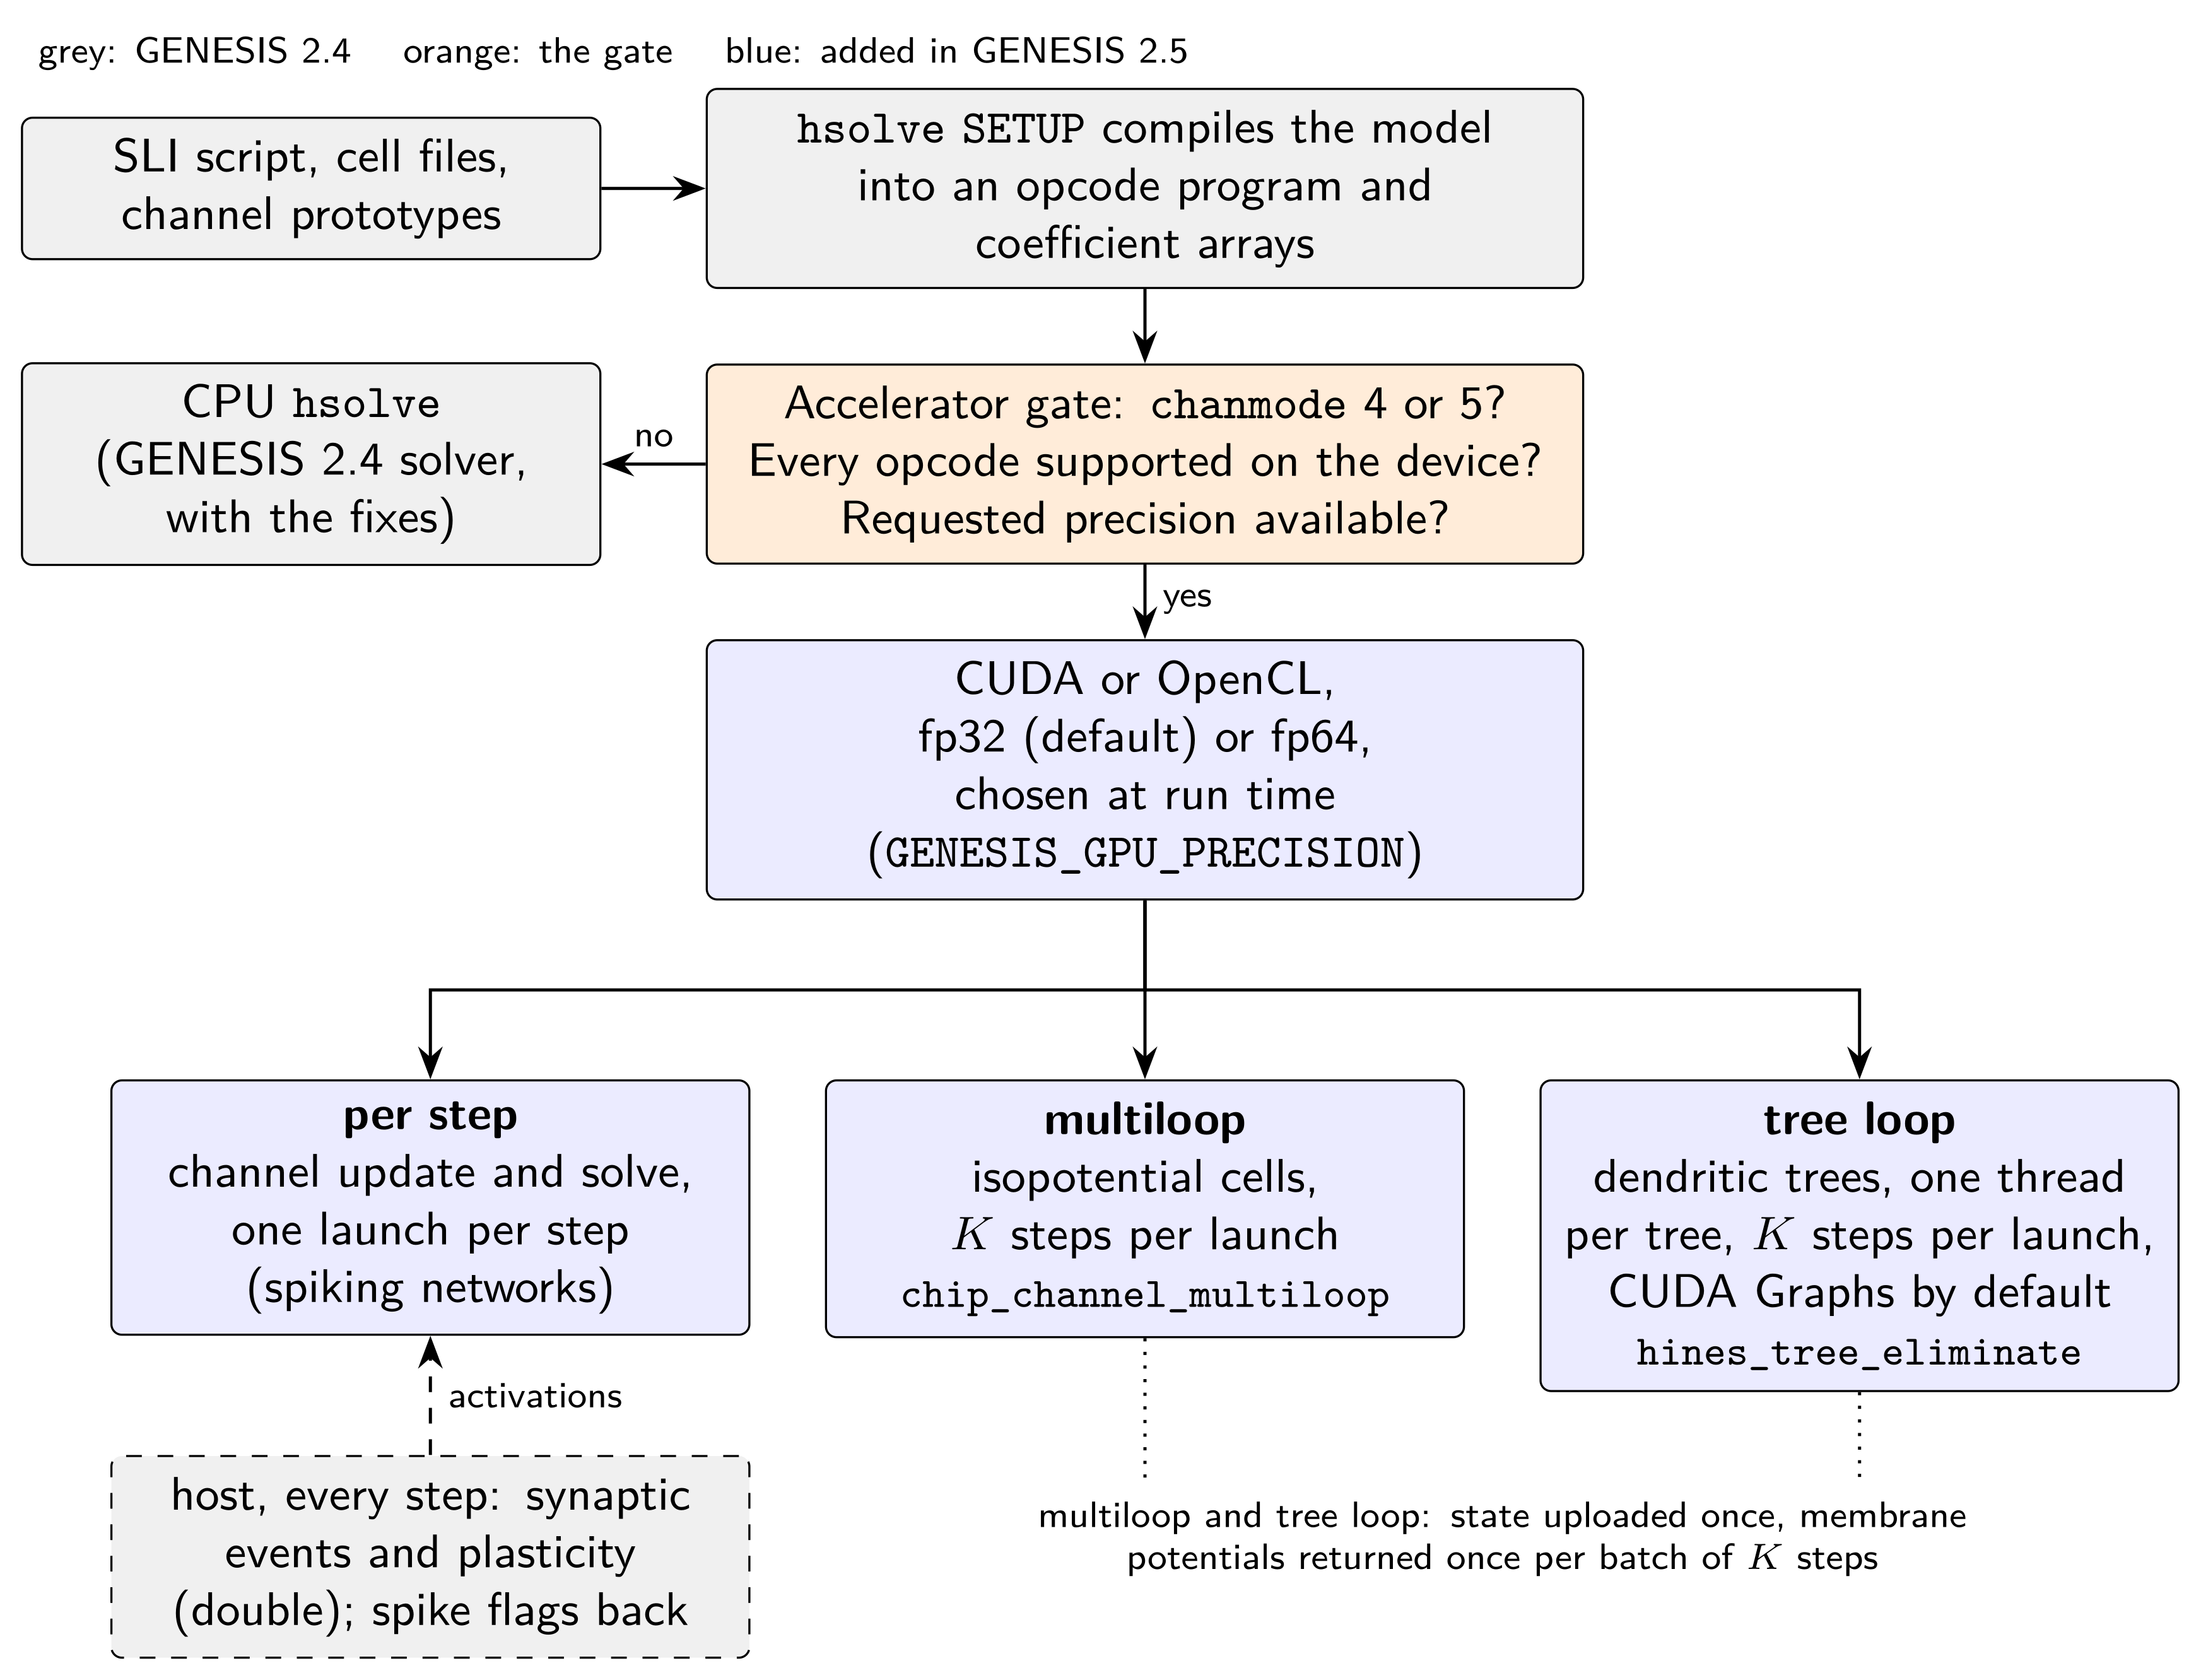
\includegraphics[width=\textwidth]{fig_architecture.png}
\caption{How a model reaches the GPU. \texttt{hsolve} compiles the model into an opcode
program at \texttt{SETUP}. A gate checks the program against what the kernels
implement; anything else stays on the CPU. Accepted models run as one of three
dispatches: per step, batched over many steps for isopotential cells
(\ccm{}), or batched for dendritic trees (\hte{}). Synaptic events are delivered by the
host every step.}
\label{fig:architecture}
\end{figure}

The backends sit behind one entry point in \texttt{hsolve}
(Fig.~\ref{fig:architecture}). The SLI interpreter, the element tree, the scheduler
and the PGENESIS MPI layer are those of GENESIS~2.4. A user selects a backend with
\texttt{chanmode} and environment variables. Nothing in a model script changes.

An accepted model runs on one of three paths. \emph{Per step}: the device updates
channels and solves each step, and the host delivers synaptic events and spikes between
steps. Networks whose cells exchange spikes take this path; on it a spike reaches some
of its targets one step later than on the CPU (Section~3(d)).
\emph{Multiloop}:
for isopotential cells without synaptic input, one launch runs $K$ steps.
\emph{Tree loop}: for populations of dendritic trees, the channel update and \hte{}
run back to back for $K$ steps. On the two batched paths the state goes to the device
once and the membrane potentials come back once per batch, so a run of $K$ steps
costs one transfer instead of $K$.

\textbf{Design decisions.}
\begin{enumerate}
\item \emph{The kernels interpret the solver's own program.} Both backends execute the
      opcode program \texttt{hsolve} already builds, so every model it accepts runs
      unchanged. GPU-native simulators generate code per mechanism instead. Interpreting
      costs divergence and a fixed setup time (Section~3); in exchange, existing
      models need no porting.
\item \emph{The tree solve needs no synchronisation.} The elimination program of a
      population is block-diagonal: each tree touches only its own rows. Each thread
      therefore runs the CPU's elimination for one tree, with no barrier. The only
      change needed was to split, per tree, the opcode that joins two trees in the CPU
      program.
\item \emph{What the kernels cannot compute is refused, not approximated.} Release v2.5,
      which the first version of this paper described, accepted models with synaptic,
      spike, GHK and concentration elements and returned plausible but wrong voltages. Such programs are now detected at
      \texttt{SETUP} and computed on the CPU.
\item \emph{The device owns the state it computes.} With synaptic input the host
      writes only the slots it owns each step. Release v2.5 uploaded the whole state,
      which overwrote gating variables the kernel had just updated.
\end{enumerate}

\textbf{Execution model.}
Four properties of the device code determine when the GPU pays off.
\emph{Work imbalance.} \hte{} runs one thread per tree, so the threads of a warp wait
for the largest tree among them. A population that mixes trees of 8 and 64
compartments in every warp takes \claim{e7_inter_over_uniform}$\times$ as long per
step as uniform trees with the same total number of compartments. The CPU pays about
the same for this mix (\claim{e7_cpu_inter_over_uniform}$\times$), so the waiting
costs little. Grouping the same trees by size is slower
(\claim{e7_block_over_uniform}$\times$, E7), because it puts all the long trees on a
few multiprocessors, which then finish last.
\emph{Divergence.} Compartments with different channel sets follow different opcode
streams through the interpreter, so heterogeneous cells cost more than their
compartment count suggests.
\emph{Transfers.} On the batched paths transfers are fixed per batch, not per step
(above). On the per-step path they are paid every step.
\emph{Launch overhead.} In the tree loop on the A100 the host needs
\claim{f2_host_us_per_step}\,\textmu s per step to launch the two kernels, which run
for \claim{f2_kernel_us_per_step}\,\textmu s (Nsight Systems, $N=10\,000$ trees). The
launches overlap the kernels and do not limit the loop. CUDA Graphs, which replay a
recorded sequence of launches, cut the host's part to
\claim{f2_host_graph_us_per_step}\,\textmu s per step. In a run of $K=50\,000$ steps
they save \claim{e8_gain_tree_k50000_a100}\,$\pm$\,\claim{e8_gain_tree_k50000_a100_sd}\%
of the run time on the A100 and
\claim{e8_gain_tree_k50000_a40}\,$\pm$\,\claim{e8_gain_tree_k50000_a40_sd}\% on the A40
(E8). At $K=5000$ they save
\claim{e8_gain_tree_k5000_a100}\,$\pm$\,\claim{e8_gain_tree_k5000_a100_sd}\% on the
A100 and \claim{e8_gain_tree_k5000_a40}\,$\pm$\,\claim{e8_gain_tree_k5000_a40_sd}\% on
the A40, which is within the noise. Graphs change no result, so they are on by default
for the tree loop. On the spiking network they make no difference within error
(\claim{e8_gain_spiking_a100}\,$\pm$\,\claim{e8_gain_spiking_a100_sd}\%). There the
cost is the host's event delivery and the synchronisation it forces every step. Moving
spike delivery to the device is the next step for that workload.

\item Software functionalities

\textbf{Precision.}
Single precision is the default. \texttt{GENESIS\_\allowbreak GPU\_\allowbreak PRECISION=fp64} selects double
precision at run time in the same binary, and a device without it refuses with a
message and computes on the CPU. In fp64 the GPU reproduces the CPU solver to every
printed digit (ten significant figures) on our verification models; in fp32 it agrees
to within \claim{fp32_single_ap_v}\,V over one action potential on every device we
tested. Synaptic weights and
plasticity are computed by the synapse objects on the host in double precision in every
mode. Only the resulting activation reaches the device. Section~3 measures the cost of
double precision on each card and compares the two precisions over a 10\,s run.
Runs longer than 10\,s, with or without plasticity, and PGENESIS runs in which several
MPI ranks share one GPU have not been tested.

\textbf{Portability.}
The OpenCL backend runs the same kernels on any OpenCL~1.2 device. We test it on the
NVIDIA A40 and A100 and on the AMD Radeon~890M integrated GPU under two independent
implementations, AMD ROCm and Mesa rusticl (E9). On the same chip the two differ:
ROCm exposes double precision and rusticl does not, so under rusticl a request for
fp64 is refused and the model computes on the CPU. On an integrated GPU that also
drives the display, a long tree dispatch trips the driver's watchdog. For that reason
the OpenCL backend declines the batched tree dispatch above \claim{ocl_igpu_tree_cap}
compartments by default, prints a message and runs the model step by step; on a
dedicated card
\texttt{GENESIS\_\allowbreak OCL\_\allowbreak TREE\_\allowbreak MAX\_\allowbreak NCOMPTS=0}
lifts the limit, as in all our measurements, and E9 checks that the limit is
enforced. Under rusticl, which
submits to the graphics queue, the same kind of limit stops the longest
single-compartment run: the driver resets the GPU during the network of $N=50\,000$
cells batched over 50\,000 steps. Run one dispatch per step, the model takes
\claim{e9_rusticl_perstep_n50000_s}\,s, slower than the laptop's CPU at
\claim{e9_t1_cpu_n50000_s}\,s, while ROCm runs it batched in
\claim{e9_t1_rocm_n50000_s}\,s. Release v2.6.1 splits such a run into dispatches of
about half a second, with the same result, so under rusticl it too runs batched on
the GPU.

\item Sample code

A model needs no change as long as its solver uses \texttt{chanmode~4} or \texttt{chanmode~5}, modes
GENESIS~2.4 already has. An existing script that builds its solver as

{\footnotesize\begin{verbatim}
create hsolve /net/solver
setfield /net/solver path "/net/##[][TYPE=compartment]" \
    chanmode 4
call /net/solver SETUP
\end{verbatim}}

runs on the GPU when started with \texttt{nxgenesis} (CUDA) or
\texttt{nxgenesis\_ocl} (OpenCL) from the release. Batching and precision are chosen
when the run starts, for example

{\footnotesize\begin{verbatim}
GENESIS_CUDA_MULTILOOP=<K> GENESIS_GPU_PRECISION=fp64 \
    nxgenesis -batch model.g
\end{verbatim}}

The start-up lines name the backend, the precision and the dispatch path in use, and
a model the device cannot compute is reported and run on the CPU.
\end{enumerate}

\item Illustrative examples

Every number in this section was measured on release v2.6.0 on the UMCS ``Lunar''
cluster (inf02: Xeon Gold 6342 and NVIDIA A40; inf03: Xeon Platinum 8358 and NVIDIA
A100). Release v2.6.2, which the metadata cite,
fixes all the defects found during the work on this paper and computes the same
results: on both cards its fp32 output is byte-identical to that of v2.6.0, and its
fp64 output agrees with the CPU solver to $10^{-10}$\,V.
CPU arms are single-threaded. Times are wall-clock times of the whole process,
and each value is a mean over replicates run in interleaved order. All runs, CPU arms
included, were bound to the GPU's NUMA node, so both arms of a speedup used the same
socket. A speedup is the ratio of two means; its uncertainty combines the two arms'
relative sample standard deviations in quadrature. On inf02 the A40's socket is the
slower one: a CPU arm takes \claim{numa_socket_penalty_inf02}$\times$ as long there as
on the other socket, so against a CPU arm on the other socket the A40's speedups would
be that much smaller. On inf03 the GPU's socket is slightly faster
(\claim{numa_socket_penalty_inf03}$\times$). The CPU arms use the same \texttt{hsolve}
mode as the GPU arms (\texttt{chanmode~4}). On the trees \texttt{chanmode~3} is faster
still by \claim{cpu_cm4_over_cm3_trees}$\times$, so against it the tree speedups would
be smaller by that factor, while \texttt{chanmode~1}, our CPU reference before this
revision, is \claim{cpu_cm1_over_cm4_trees}$\times$ slower with the same voltages.

\begin{enumerate}
\item Speed on populations of cells

Table~\ref{tab:single} gives the speedups for the single-compartment network, and
Fig.~\ref{fig:trees} those for the dendritic trees, end to end and for the step phase
alone. The end-to-end gain grows with run length as the fixed setup cost is amortised
(Fig.~\ref{fig:runlength}). On the longest run of Fig.~\ref{fig:runlength} the speedup
is \claim{e2_max_e2e_a40}$\times$ on the A40 and \claim{e2_max_e2e_a100}$\times$ on the
A100. Double precision takes \claim{e2_fp64_cost_a40}$\times$ the fp32 time on the A40
and \claim{e2_fp64_cost_a100}$\times$ on the A100.

\begin{table}[!h]
\centering\small
\begin{tabular}{rcccc}
\toprule
 & \multicolumn{2}{c}{NVIDIA A40} & \multicolumn{2}{c}{NVIDIA A100} \\
$N$ & CUDA & OpenCL & CUDA & OpenCL \\
\midrule
500 & \claim{e3_t1_cuda_a40_n500}\,$\pm$\,\claim{e3_t1_cuda_a40_n500_sd} & \claim{e3_t1_ocl_a40_n500}\,$\pm$\,\claim{e3_t1_ocl_a40_n500_sd} & \claim{e3_t1_cuda_a100_n500}\,$\pm$\,\claim{e3_t1_cuda_a100_n500_sd} & \claim{e3_t1_ocl_a100_n500}\,$\pm$\,\claim{e3_t1_ocl_a100_n500_sd} \\
5\,000 & \claim{e3_t1_cuda_a40_n5000}\,$\pm$\,\claim{e3_t1_cuda_a40_n5000_sd} & \claim{e3_t1_ocl_a40_n5000}\,$\pm$\,\claim{e3_t1_ocl_a40_n5000_sd} & \claim{e3_t1_cuda_a100_n5000}\,$\pm$\,\claim{e3_t1_cuda_a100_n5000_sd} & \claim{e3_t1_ocl_a100_n5000}\,$\pm$\,\claim{e3_t1_ocl_a100_n5000_sd} \\
50\,000 & \claim{e3_t1_cuda_a40_n50000}\,$\pm$\,\claim{e3_t1_cuda_a40_n50000_sd} & \claim{e3_t1_ocl_a40_n50000}\,$\pm$\,\claim{e3_t1_ocl_a40_n50000_sd} & \claim{e3_t1_cuda_a100_n50000}\,$\pm$\,\claim{e3_t1_cuda_a100_n50000_sd} & \claim{e3_t1_ocl_a100_n50000}\,$\pm$\,\claim{e3_t1_ocl_a100_n50000_sd} \\
\bottomrule
\end{tabular}
\caption{Single-compartment network, $K=50\,000$ steps: speedup of each backend over
the CPU solver (E3, 10 replicates).}
\label{tab:single}
\end{table}

\begin{figure}[!h]
\centering
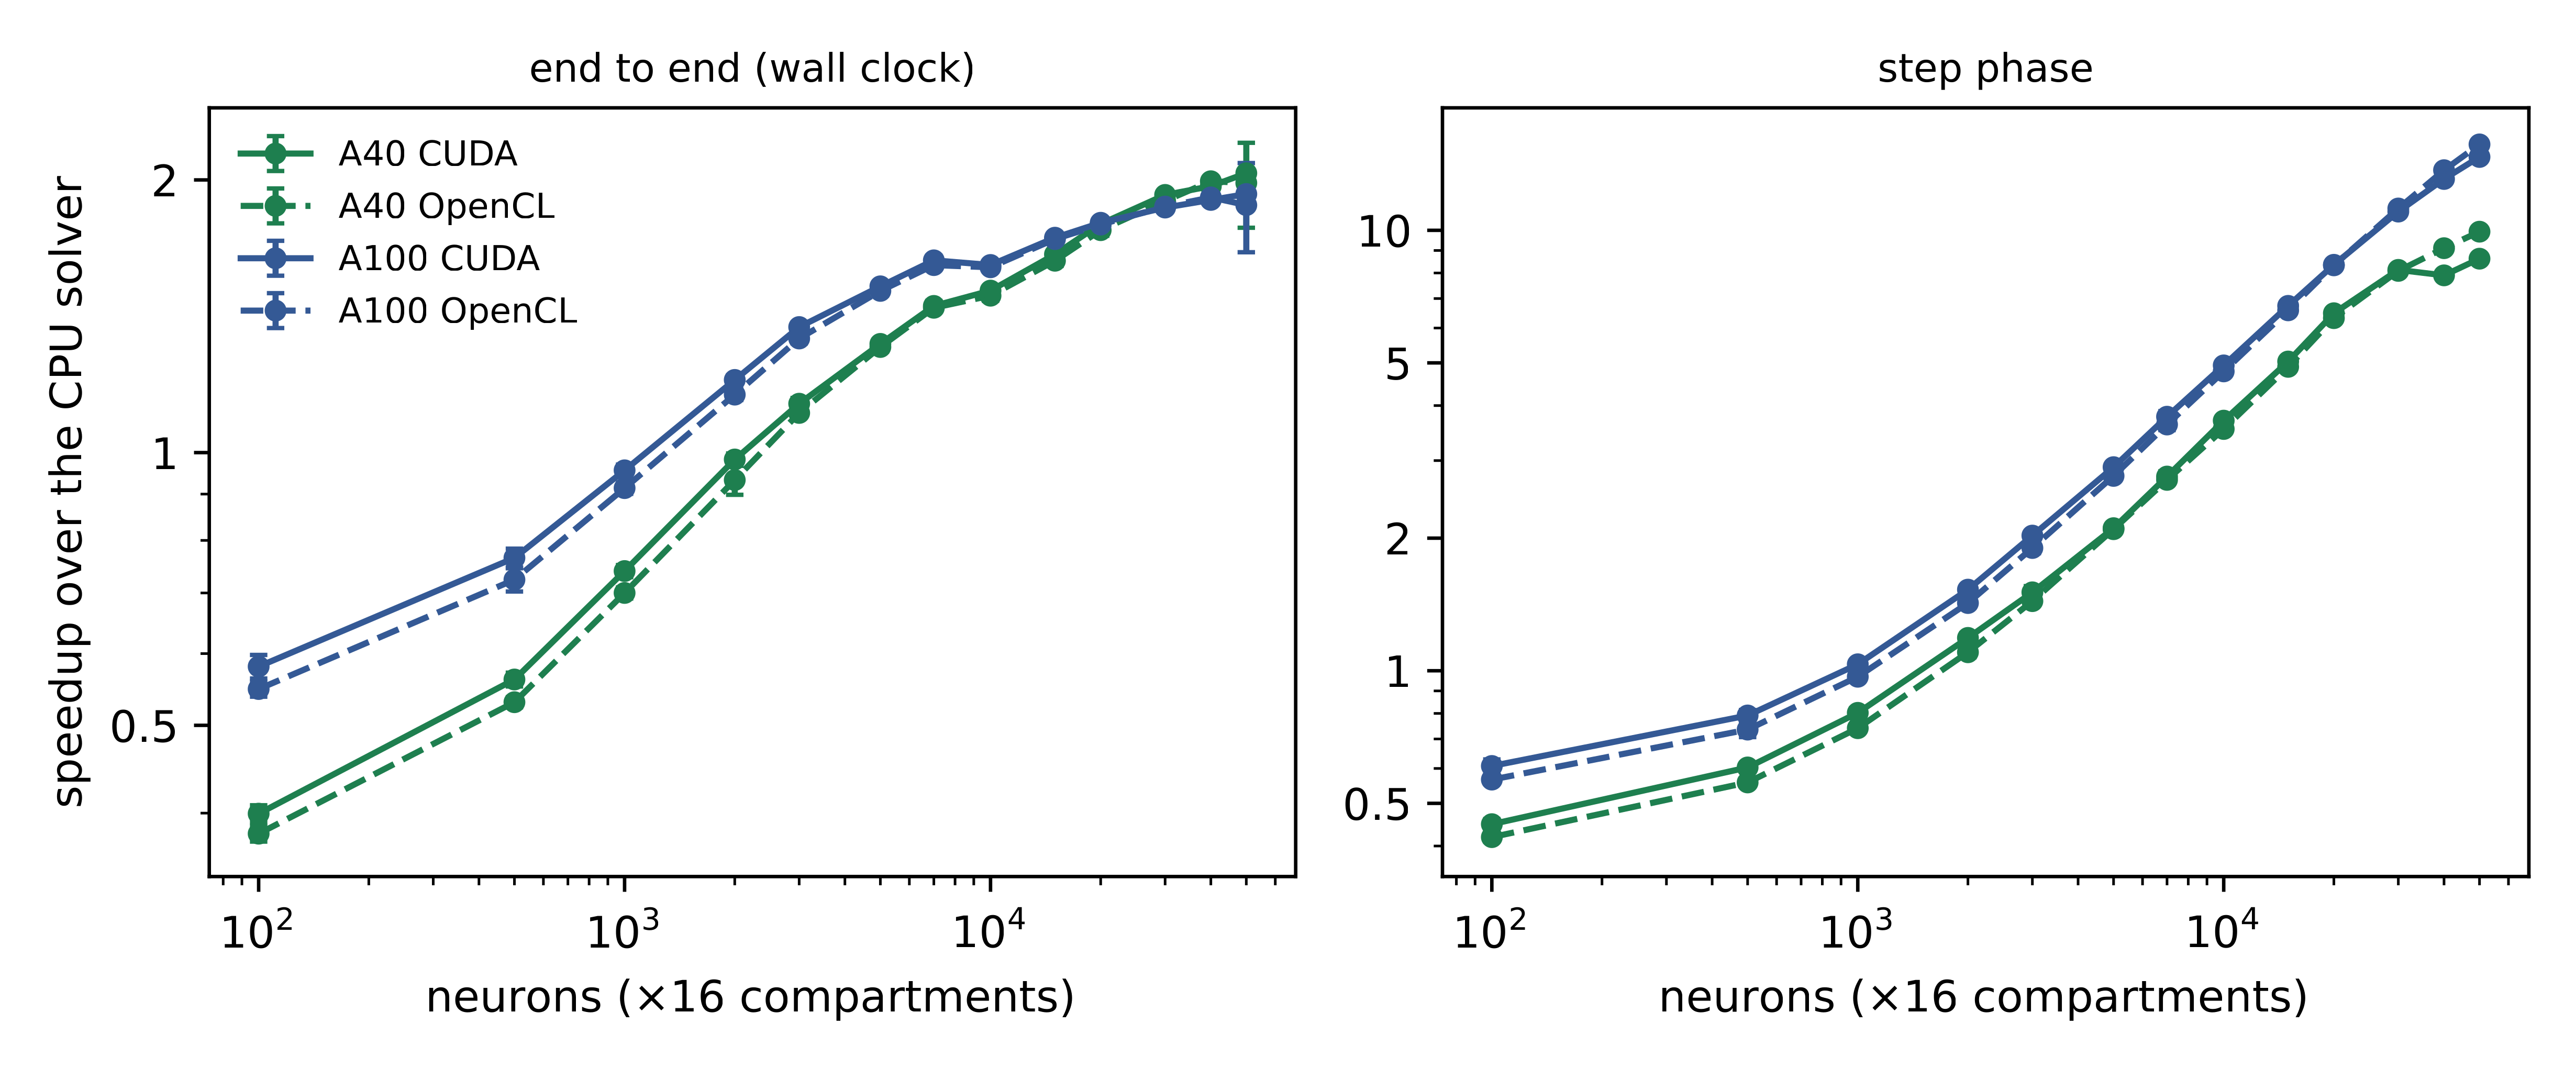
\includegraphics[width=\textwidth]{fig_trees.png}
\caption{Dendritic trees, $N\times16$ compartments, 200 steps: speedup over the CPU
solver, end to end and step phase, on the A40 and A100 (E3).}
\label{fig:trees}
\end{figure}

\begin{figure}[!h]
\centering
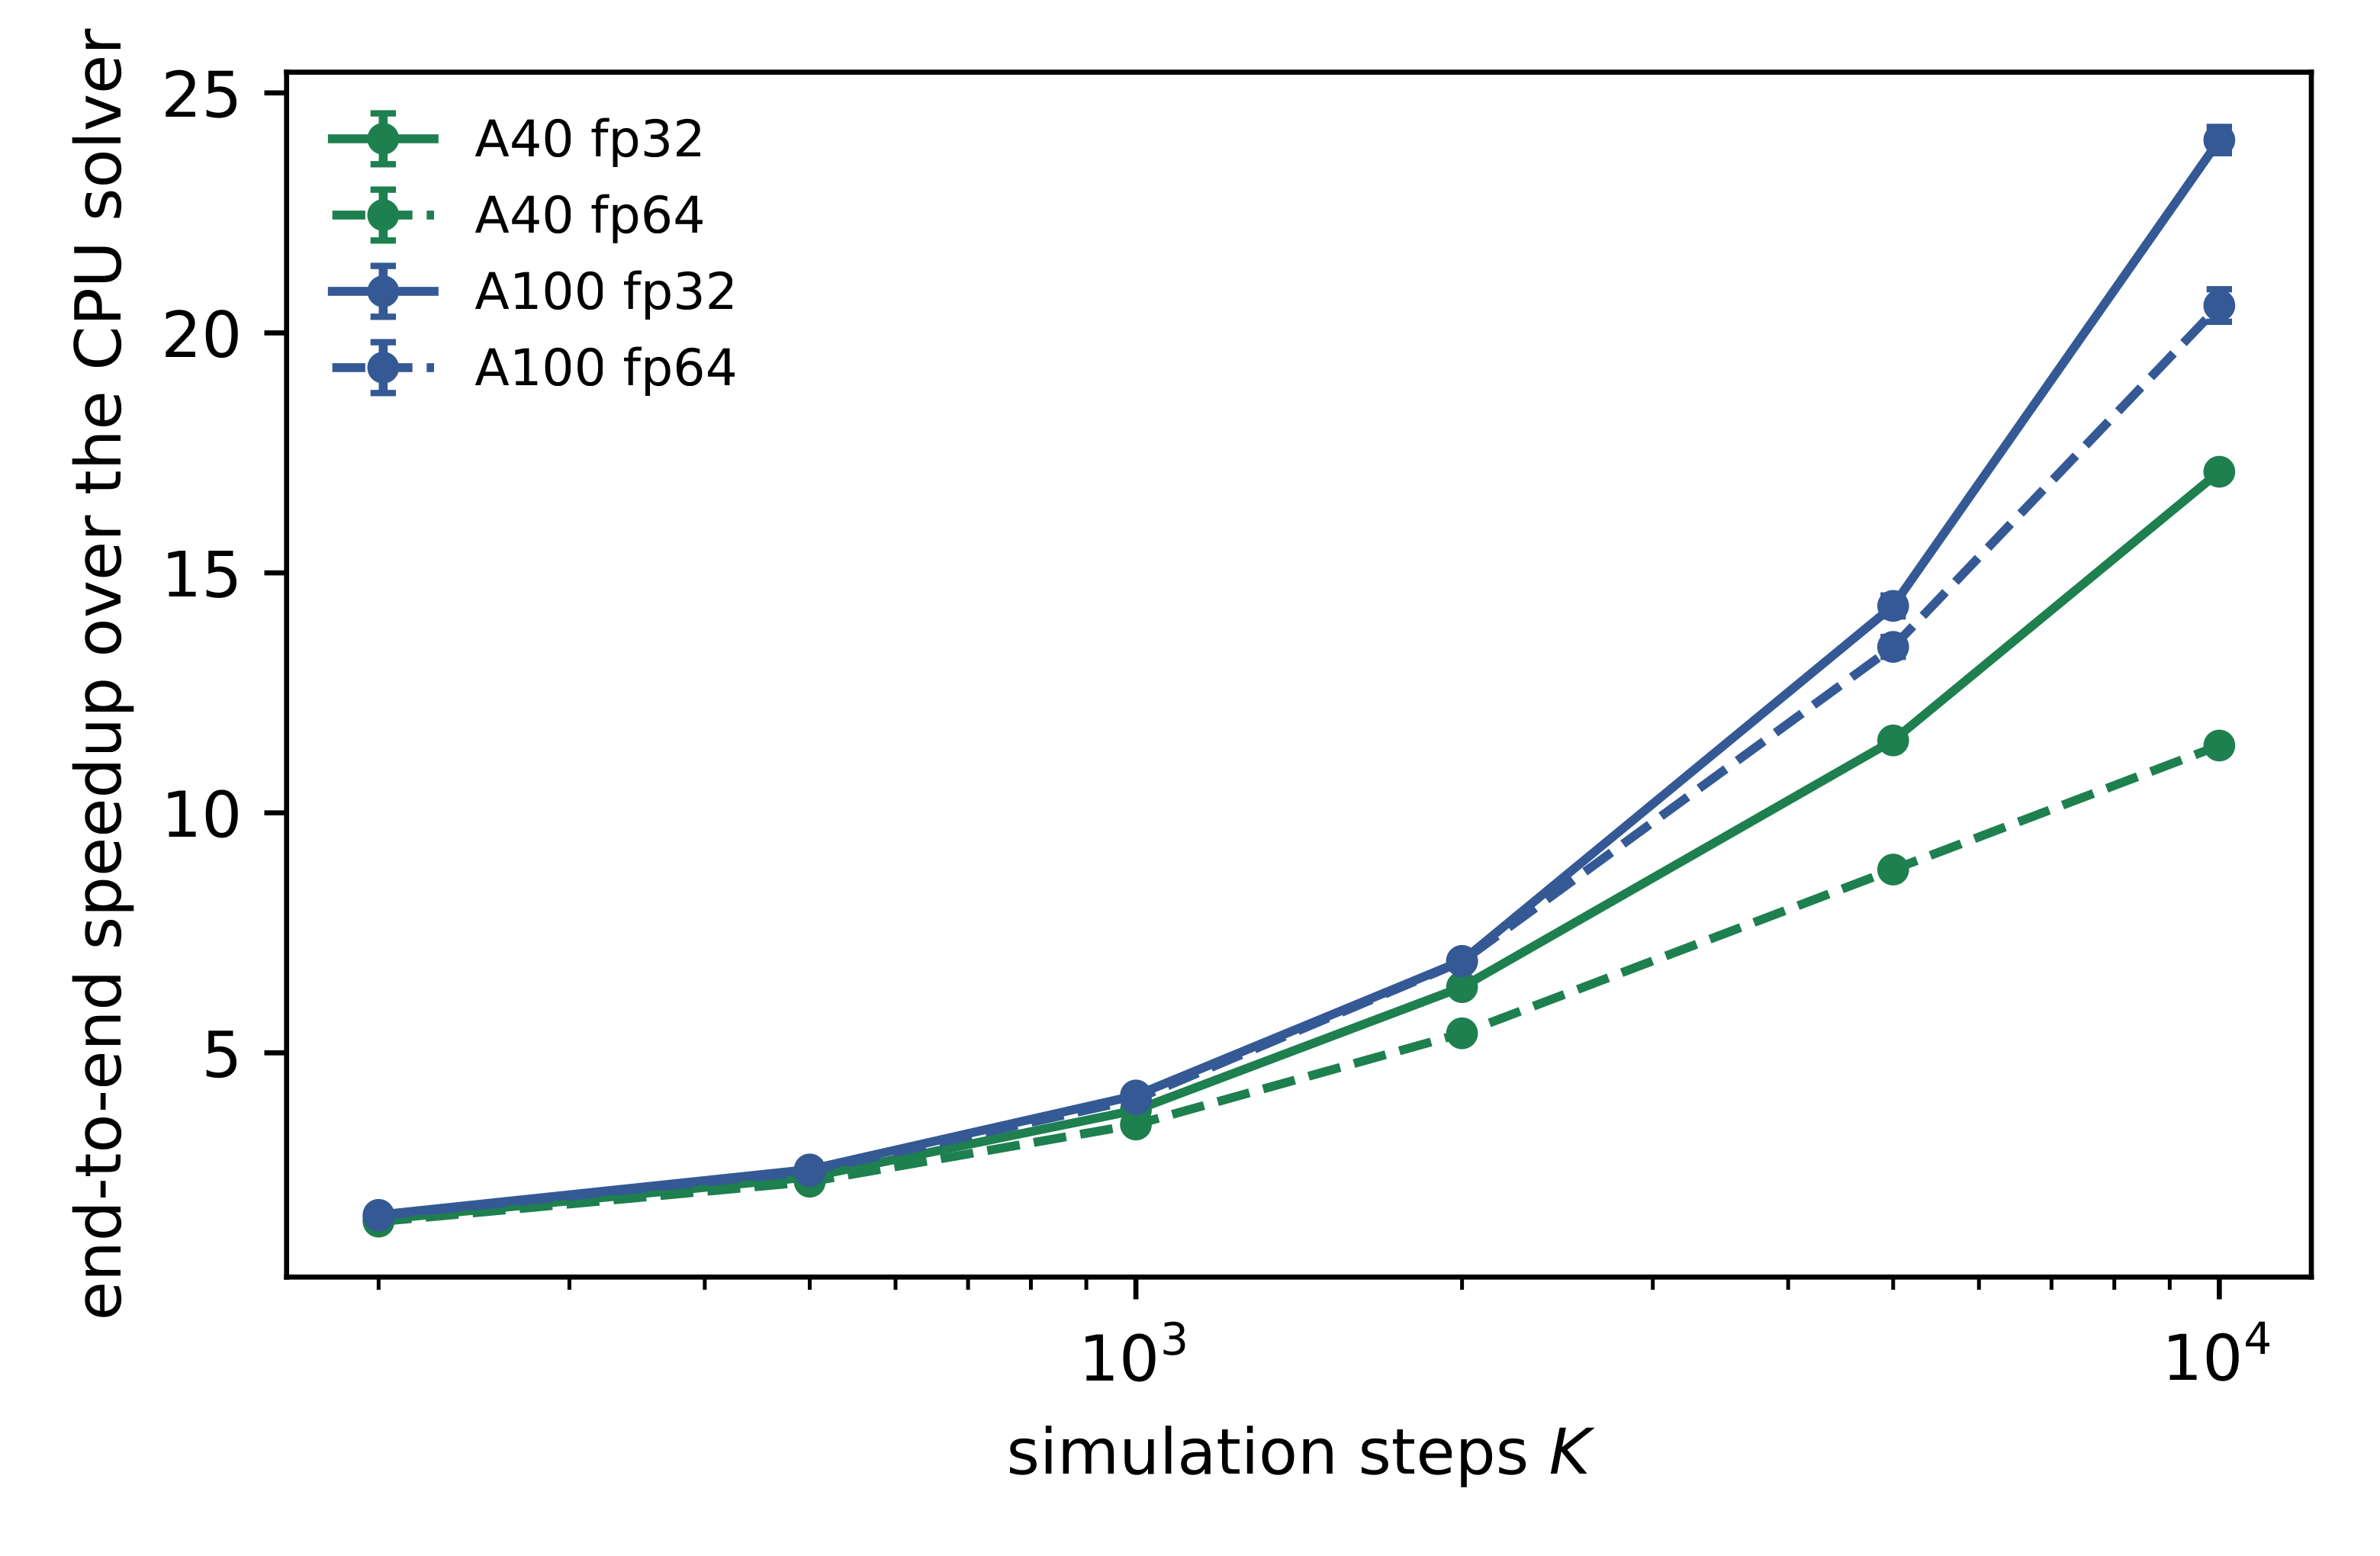
\includegraphics[width=0.62\textwidth]{fig_runlength.png}
\caption{End-to-end speedup against run length, $10\,000\times16$ compartments, fp32
and fp64, both cards (E2).}
\label{fig:runlength}
\end{figure}

\item Against other simulators

Table~\ref{tab:sim} lists every arm of the spiking-network comparison, measured in
one session on one node in interleaved order, so no ratio in it mixes machines or
days. Arbor cannot express the benchmark's zero axonal delay, so its arm uses a delay
of one step (50\,\textmu s). Arbor advances in epochs of half the shortest connection
delay and exchanges spikes once per epoch~\cite{arbor_docs_epochs}; with this delay it
does so at least once per step, the same per-step exchange that keeps GENESIS from
gaining on the GPU. We did not profile Arbor to confirm that this is where its time
goes.

On the dendritic trees GENESIS pays more than Arbor at setup and less per step. In
single precision it is slower than Arbor on short runs and faster beyond
\claim{e4_crossover_ms_a100}\,ms of simulated time on the A100 and
\claim{e4_crossover_ms_a40}\,ms on the A40; at the longest run it takes
\claim{e4_g32_over_arbor_a100}$\times$ Arbor's time on the A100 and
\claim{e4_g32_over_arbor_a40}$\times$ on the A40 (Fig.~\ref{fig:crossover}). In double
precision, which Arbor always uses, GENESIS is slower at every run length we measured,
taking \claim{e4_fp64_over_arbor_a100}$\times$ Arbor's time on the A100 and
\claim{e4_fp64_over_arbor_a40}$\times$ on the A40 at the longest run.

We profiled GENESIS and CoreNEURON on one CPU core (E6). GENESIS is faster on both
workloads, \claim{e6_cn_over_g_spk}$\times$ on the network and
\claim{e6_cn_over_g_tree}$\times$ on the trees. GENESIS reads its channel gates from
tables; CoreNEURON evaluates exponentials, and the exponential function alone takes
\claim{e6_cn_spk_libm}\% of its time on the network. On the network GENESIS spends
\claim{e6_g_spk_syn_disp}\% of its time on synapses, spike events and the calls that
reach them, against CoreNEURON's \claim{e6_cn_spk_syn}\%. This host-side work runs on
the CPU every step, so the GPU cannot speed it up. On the trees the channels take
\claim{e6_g_tree_chan}\% of GENESIS's time and the linear solve
\claim{e6_g_tree_solve}\%, against \claim{e6_cn_tree_chan}\% and
\claim{e6_cn_tree_solve}\% of CoreNEURON's. Most of the rest is model construction in
both, plus idle library threads in CoreNEURON.

\begin{table}[!h]
\centering\small
\begin{tabular}{>{\raggedright\arraybackslash}p{5.6cm}lrr}
\toprule
Simulator & Hardware & Wall time (s) & Relative \\
\midrule
GENESIS 2.5, one solver per cell (as published) & CPU & \claim{e1_g_cpu_pub_s}\,$\pm$\,\claim{e1_g_cpu_pub_s_sd} & \claim{e1_g_cpu_pub_rel} \\
GENESIS 2.5, one solver per layer & CPU & \claim{e1_g_cpu_1s_s}\,$\pm$\,\claim{e1_g_cpu_1s_s_sd} & 1 \\
GENESIS 2.5, one solver per layer, fp32 & A100 & \claim{e1_g_gpu32_1s_s}\,$\pm$\,\claim{e1_g_gpu32_1s_s_sd} & \claim{e1_g_gpu32_1s_rel} \\
GENESIS 2.5, one solver per layer, fp64 & A100 & \claim{e1_g_gpu64_1s_s}\,$\pm$\,\claim{e1_g_gpu64_1s_s_sd} & \claim{e1_g_gpu64_1s_rel} \\
NEURON 9.0.2, NMODL channels & CPU & \claim{e1_nrn_cpu_s}\,$\pm$\,\claim{e1_nrn_cpu_s_sd} & \claim{e1_nrn_cpu_rel} \\
NEURON 9.0.2, ChannelBuilder channels & CPU & \claim{e1_nrn_cb_cpu_s}\,$\pm$\,\claim{e1_nrn_cb_cpu_s_sd} & \claim{e1_nrn_cb_cpu_rel} \\
CoreNEURON 9.0.2 & CPU & \claim{e1_cn_cpu_s}\,$\pm$\,\claim{e1_cn_cpu_s_sd} & \claim{e1_cn_cpu_rel} \\
CoreNEURON 9.0.2 & A100 & \claim{e1_cn_gpu_s}\,$\pm$\,\claim{e1_cn_gpu_s_sd} & \claim{e1_cn_gpu_rel} \\
Arbor 0.10.0 & A100 & \claim{e1_arbor_gpu_s}\,$\pm$\,\claim{e1_arbor_gpu_s_sd} & \claim{e1_arbor_gpu_rel} \\
\bottomrule
\end{tabular}
\caption{Vogels--Abbott COBAHH network~\cite{vogels2005signal,brette2007simulation},
4000 cells, 5\,s: wall time of every arm in one session on inf03 (E1, 5 replicates,
interleaved). Relative: wall time over that of GENESIS with one solver per layer on
the CPU; below 1 is faster.}
\label{tab:sim}
\end{table}

\begin{figure}[!h]
\centering
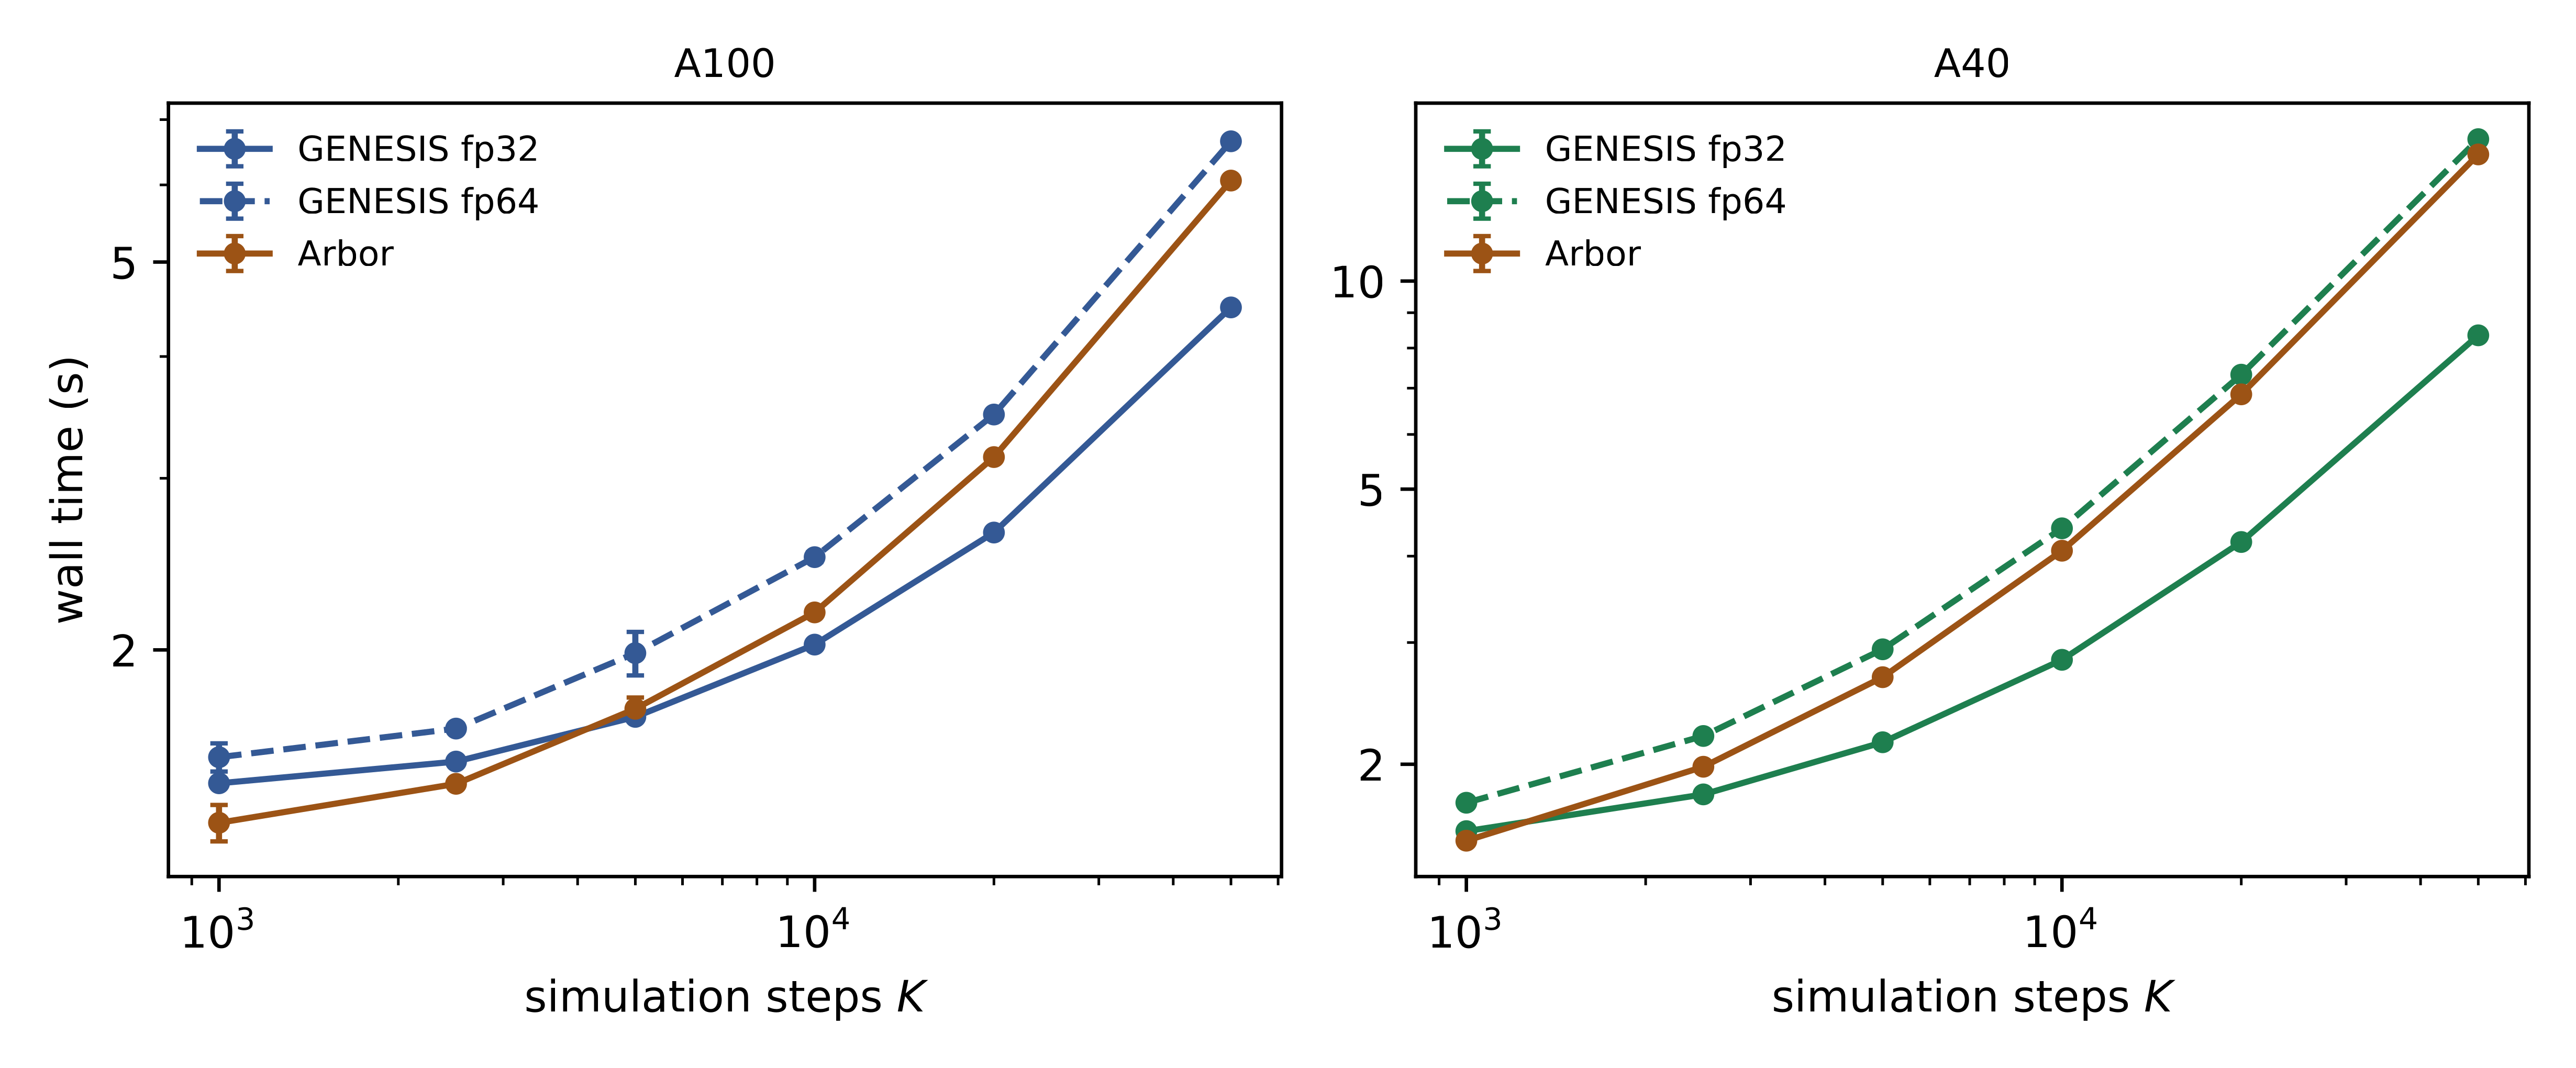
\includegraphics[width=\textwidth]{fig_crossover.png}
\caption{GENESIS and Arbor on the same GPU against run length, GENESIS in fp32 and fp64
(E4).}
\label{fig:crossover}
\end{figure}

\item When to use the GPU

Table~\ref{tab:regimes} gathers what the measurements above say about where the
accelerator pays off and where it does not.
\begin{table}[!h]
\centering\small
\begin{tabular}{>{\raggedright\arraybackslash}p{4cm}>{\raggedright\arraybackslash}p{2.6cm}>{\raggedright\arraybackslash}p{5.8cm}}
\toprule
Workload & GPU? & Why \\
\midrule
One detailed morphology, or fewer than about \claim{regime_trees_min_n} trees & No & too few trees to fill the device; below the threshold the GPU is slower (Fig.~\ref{fig:trees}) \\
Population of dendritic trees & Yes, from about \claim{regime_trees_min_n} cells (200 steps) & many trees fill the device (Fig.~\ref{fig:trees}) \\
Isopotential cells without synapses & Yes & \claim{regime_single_max}$\times$ at $N=50\,000$ (Table~\ref{tab:single}) \\
Spiking network, zero axonal delay & No: \claim{e1_g_gpu32_1s_rel}$\times$ slower & spikes are exchanged every step, so every step is a dispatch (Table~\ref{tab:sim}) \\
Long runs & Gain grows with length & the fixed setup cost is amortised (Fig.~\ref{fig:runlength}) \\
\bottomrule
\end{tabular}
\caption{Where acceleration helps.}
\label{tab:regimes}
\end{table}

\item Correctness over a long run

The GPU and CPU solvers do not order spikes the same way. On the GPU a spike emitted
in one step reaches its targets in the next; the CPU solver delivers it within the step
to the cells after the sender in its loop. With this network's zero axonal delay the
two schedules differ by one step (50\,\textmu s) for some synapses, and the network is
chaotic, so it amplifies the difference. Over 10\,s of the spiking network, twice the
length of any comparison above, the GPU's spike train first departs from the CPU's
after \claim{e5_div_g64_ms}\,ms, in fp64 and in fp32 alike.
The two precisions part at the same step, so the cause is the order, not rounding. The
CPU is just as sensitive to its own order: with one solver per cell instead of one per
layer, the same network and seed depart from the first CPU run after
\claim{e5_div_pcell_ms}\,ms. From then on only statistics can be compared. Against
the CPU's \claim{e5_rate_cpu_hz}\,Hz, the spike count differs by
\claim{e5_count_g64_pct}\% in fp64, \claim{e5_count_g32_pct}\% in fp32 and
\claim{e5_count_pcell_pct}\% for the CPU in the other order; the KS distances
between the interspike-interval distributions are \claim{e5_ks_g64},
\claim{e5_ks_g32} and \claim{e5_ks_pcell}. Four other seeds, other draws of the
same network, fire at \claim{e5_rate_seed_min_hz}--\claim{e5_rate_seed_max_hz}\,Hz
with KS distances of \claim{e5_ks_seed_min}--\claim{e5_ks_seed_max}. Each run
repeats spike for spike on its own backend. So the GPU's spike count differs from the
CPU's about as much as the CPU's own count changes under another update order. Its
interspike intervals are closer to the CPU's than that run's are, and both differences
are far smaller than the change from one draw of the network to another.

\item Reproducing these results

Each number in this paper has a row in \path{reproduce/claims.csv} that names its data
file, the rows and formula it comes from, and the script that measures it; a number
taken from the literature names its source. \path{make_numbers.py} computes the values
in the text from those files, and a lint lists any number typed by hand.
\texttt{sh reproduce/run\_all.sh} runs the stages that measured them on the reader's
hardware and computes the same numbers from the new data with the same code, beside
the published ones: about 14 minutes on an A100, build included, for
Table~\ref{tab:single}, the run-length speedup and CUDA Graphs, and about 70 minutes
at the paper's full sizes (NVIDIA GPU, CUDA~12.x). Run so from a fresh clone, the
10\,s simulations of Section~3(d) gave back the published spike trains spike for
spike. With \texttt{--cpu-only} it measures the results that need no GPU in
about three minutes on any Linux machine, and the same path runs in a container (\texttt{docker build -t genesis25-cpu . \&\& docker run
--rm genesis25-cpu}) with nothing else installed, as in our earlier pipeline for
GENESIS experiments~\cite{chlasta2023pipeline}. Both run in the repository's CI on every
commit. A generated table in the README says which results need which hardware. The
comparison simulators and the reference model are built by committed recipes with
pinned versions and checksums. Rebuilding them from an empty directory reproduced the
published CoreNEURON GPU run to the spike.
\end{enumerate}

\item Impact

Two of the release's changes help every GENESIS user, with or without a GPU. The
first is the solver fixes. In GENESIS~2.4, several cells under one \texttt{hsolve}
silently gave wrong voltages under backward Euler: the first cell's were perturbed and
the others were never computed. Under Crank--Nicolson the solve diverged or crashed.
Networks are often built this way, so published results may be affected. GENESIS~2.5
computes each cell exactly as if it were alone, which a committed test checks against
a single-cell reference. A third defect stored, for a cell of one compartment under
\texttt{chanmode~2}, the backward-Euler solution minus the previous voltage in place of
the voltage. The fixes and their tests are open as a pull request to the original
project (Section~1).

The second is construction. Building a model took time quadratic in its size, growing
as compartments$^{\claim{e3c_before_exponent_inf03}}$: 272\,000 compartments took
\claim{e3c_before_272k_min} minutes to build, and at that rate the
1.7-million-compartment population of Fig.~\ref{fig:construction} would take about
\claim{e3c_before_1700k_h} hours. Four scans of the element tree are now constant- or
linear-time. Construction grows as compartments$^{\claim{e3c_construction_exponent}}$,
and the same population builds in \claim{e3c_construction_1700k_s}\,s.
This holds for models built element by element, the common case; copying a whole
prototype cell thousands of times under one parent is still quadratic. That population
has 100\,000 cells of 17 compartments, about three times the
\claim{markram_microcircuit_neurons} neurons of a reconstructed neocortical
microcircuit~\cite{markram2015reconstruction}, though with far simpler cells. With the
tree kernel, population studies such as parameter sweeps over thousands of
morphological neurons can run on a workstation instead of in a cluster queue, in the
simulator the models were written for. Table~\ref{tab:regimes} lists the practical
regimes, including where the GPU does not help.

Two parts of this work apply beyond GENESIS. The first is the refusal rule: a backend
that cannot compute a model should say so and leave it to the CPU. Release v2.5
approximated such models and returned plausible but wrong voltages. The second is the
reproduction mechanism, a map from every published number to its raw data that
regenerates the text and runs in CI. It does not depend on GENESIS and would serve any
computational paper.

\begin{figure}[!h]
\centering
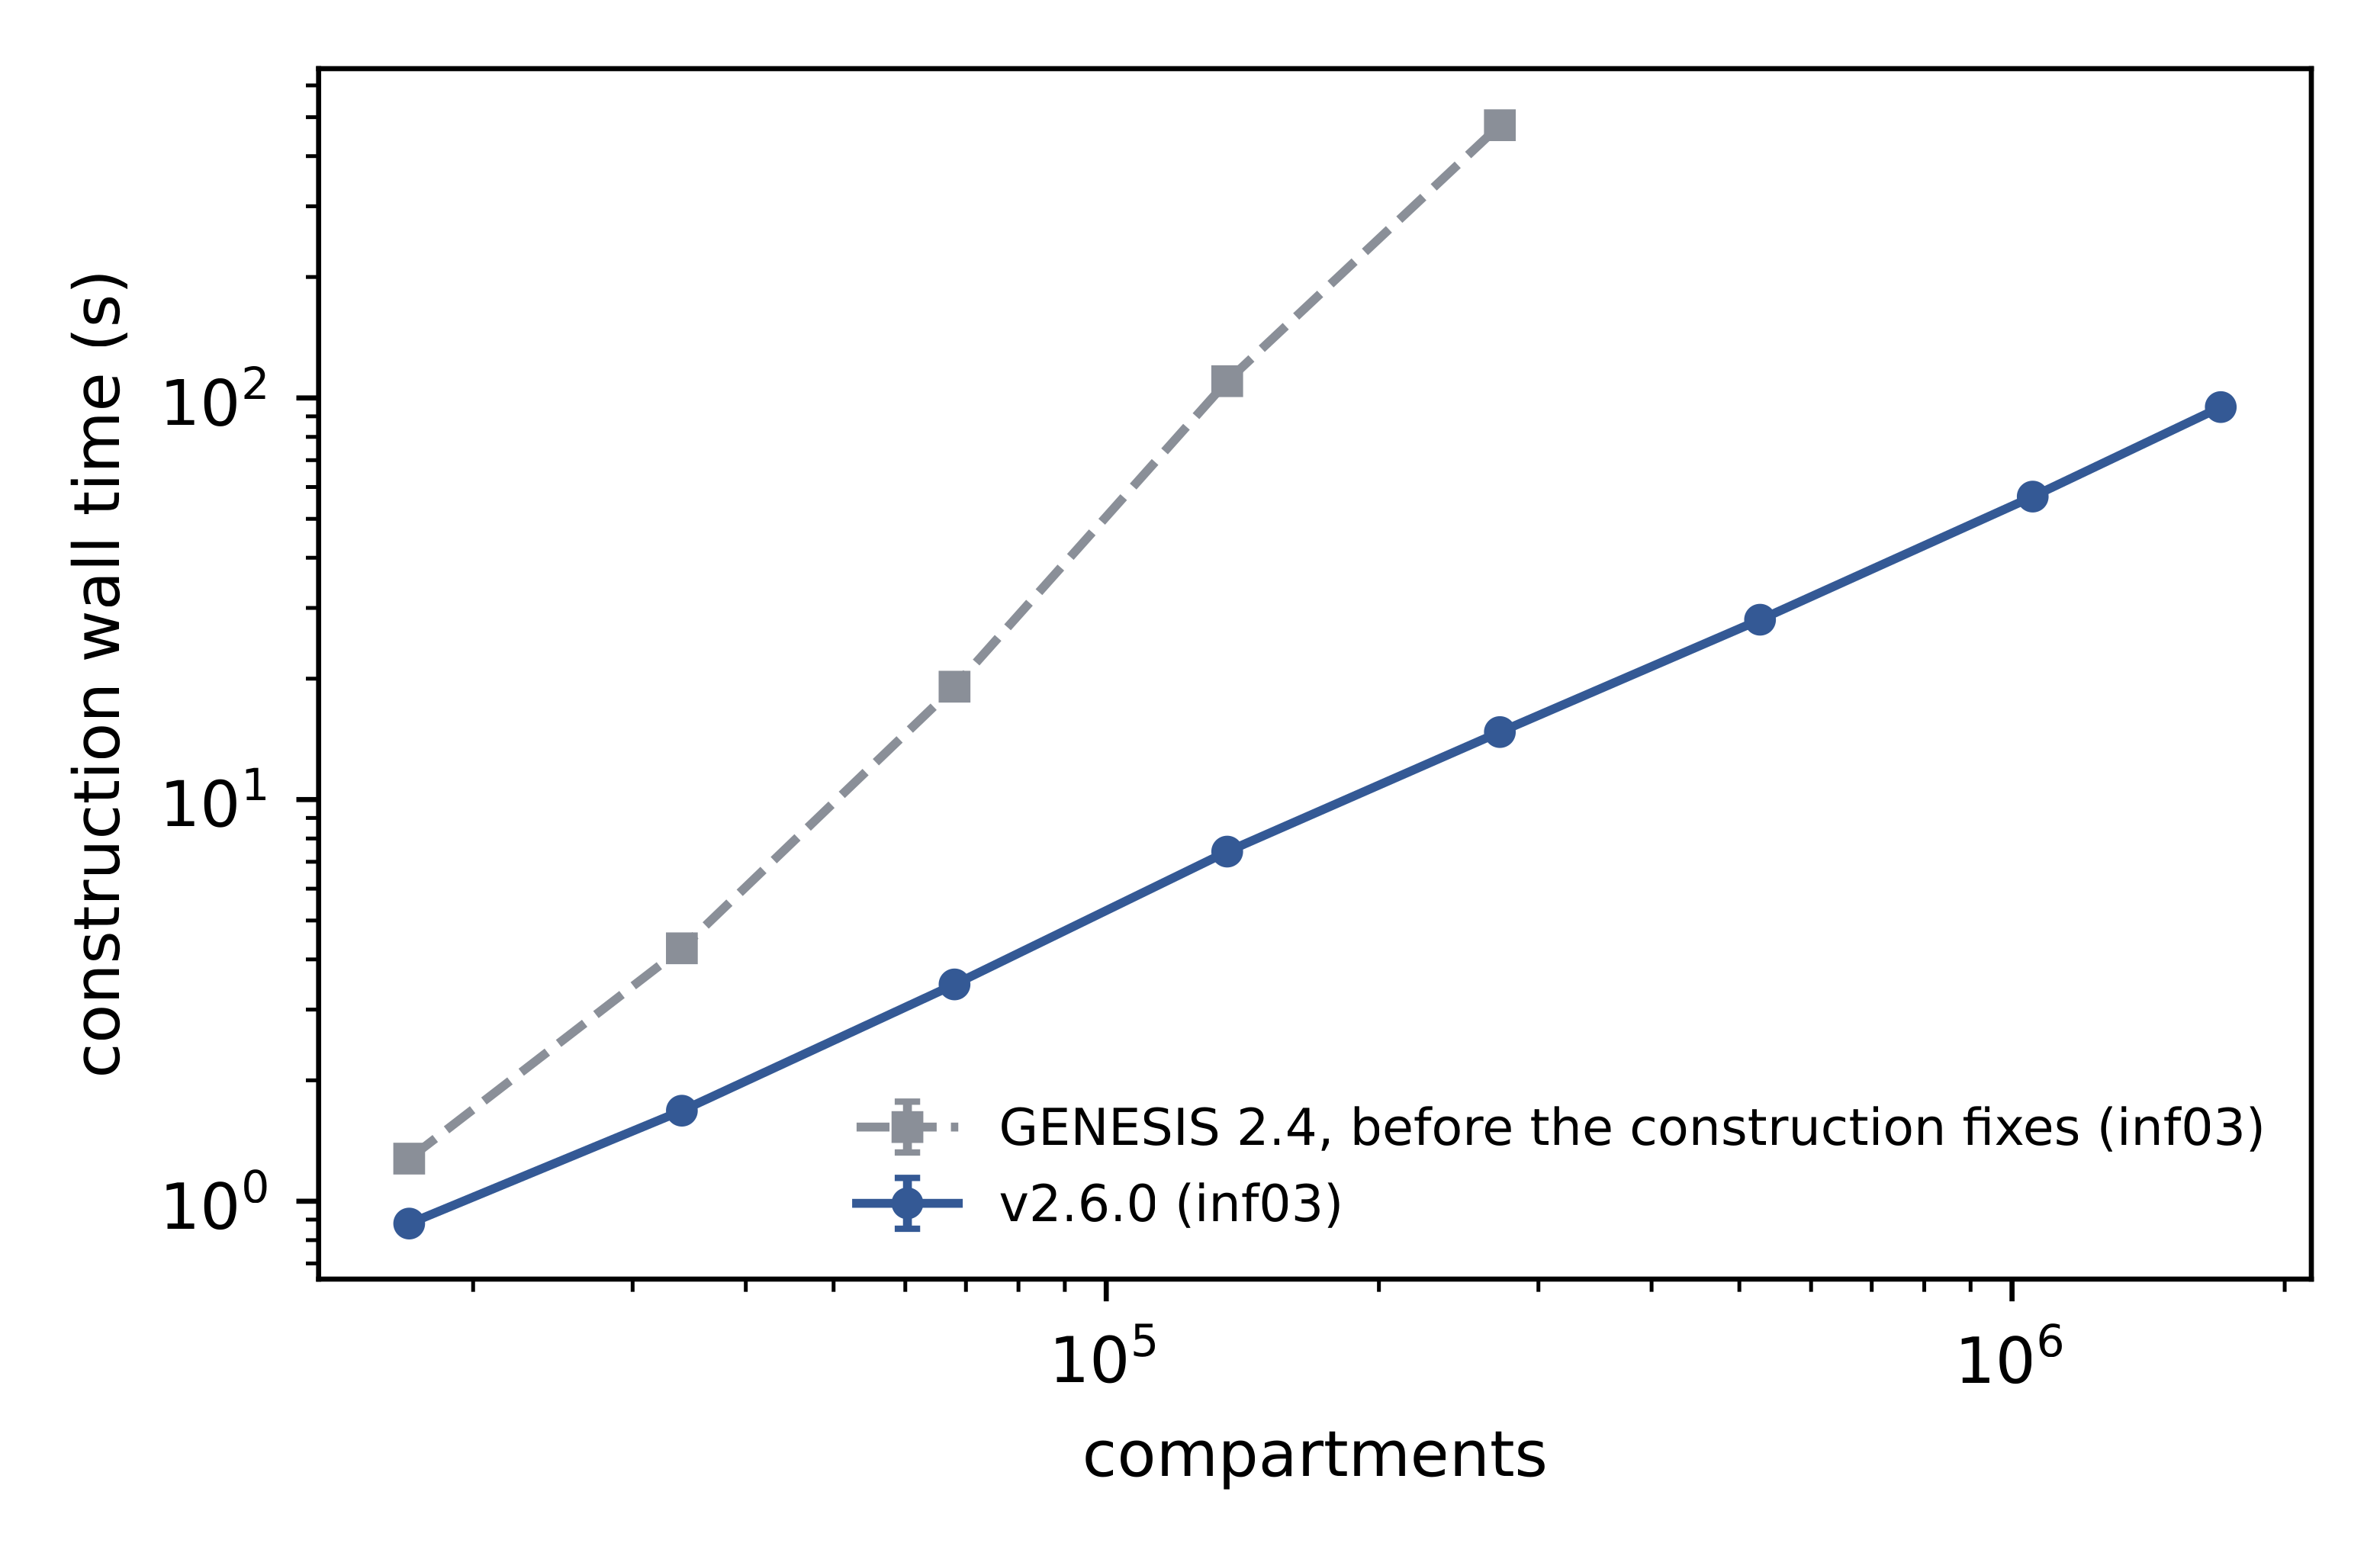
\includegraphics[width=0.62\textwidth]{fig_construction.png}
\caption{Model construction time against model size on inf03, 3 replicates each:
GENESIS~2.4 before the construction fixes (the upstream branch without them, built
on the node and timed the same way) and v2.6.0 (E3c). The code from before the fixes
was measured up to 16\,000 cells, where one build already takes
\claim{e3c_before_272k_min} minutes.}
\label{fig:construction}
\end{figure}

\item Conclusions

GENESIS~2.5 runs existing GENESIS models on a GPU with no change to their SLI scripts,
cell files or MPI workflows. The CUDA and OpenCL kernels execute \texttt{hsolve}'s own
compiled program, in single or double precision chosen at run time. Populations of
dendritic trees gain the most, up to \claim{e2_max_e2e_a100}$\times$ end to end. Single
detailed morphologies and zero-delay spiking networks run slower on the GPU: the first
has too few trees to fill the device, and the second needs host-side event delivery
every step. For spiking networks the next step is spike delivery on the device. The
solver and construction fixes help every GENESIS user and are open as a pull request to
the original project. Every measured number in this paper can be regenerated from raw
data in the repository, the hardware-independent ones on any Linux machine or in a
container.

\end{enumerate}

\section*{CRediT authorship contribution statement}

\textbf{Karol Chlasta}: Conceptualization, Data curation, Formal analysis,
Investigation, Methodology, Project administration, Resources, Software,
Validation, Visualization, Writing -- original draft, Writing -- review and
editing.
\textbf{Grzegorz Marcin W\'ojcik}: Resources, Supervision,
Writing -- review and editing.

\section*{Declaration of competing interest}

The authors declare that they have no known competing financial interests or
personal relationships that could have appeared to influence the work reported
in this paper.

\section*{Declaration of generative AI and AI-assisted technologies in the manuscript preparation process}

The authors used Anthropic's Claude to draft and edit the text and to help with the software and its benchmarks. They reviewed and edited all of it and take full responsibility for the published article.

\section*{Funding}

This research did not receive any specific grant from funding agencies in the
public, commercial, or not-for-profit sectors.

\section*{Acknowledgements}

The authors thank Maria Curie-Sk\l{}odowska University (UMCS) in Lublin and its
LubMAN computing centre for access to the ``Lunar'' cluster~\cite{umcs_lunar2015};
Karol S.~Karpowicz and Prof.~Przemys\l{}aw Stpiczy\'nski for setting up and supporting
the compute environment; and WarsawIQ for the AMD Radeon~890M on which the OpenCL
backend was developed.

% The reference list, shared by the manuscript and its revision.
\begin{thebibliography}{9}

\bibitem{bower1998}
Bower~JM, Beeman~D.
\textit{The Book of GENESIS: Exploring Realistic Neural Models with the GEneral NEural SImulation System}.
Springer, 1998.

\bibitem{hines1984efficient}
Hines~M.
Efficient computation of branched nerve equations.
\textit{International Journal of Bio-Medical Computing} 1984, 15(1):69--76. doi:10.1016/0020-7101(84)90008-4.

\bibitem{cornelis2007dendrite}
Cornelis~H, Lu~H, Esquivel~A, Bower~JM.
Modeling a single dendritic compartment using Neurospaces and GENESIS-3.
\textit{BMC Neuroscience} 2007, 8(Suppl 2):P3.

\bibitem{cornelis2008cbi}
Cornelis~H, Edwards~M, Coop~AD, Bower~JM.
The CBI architecture for computational simulation of realistic neurons and circuits in the GENESIS 3 software federation.
\textit{BMC Neuroscience} 2008, 9(Suppl 1):P88.

\bibitem{cornelis2011}
Cornelis~H, Coop~AD, Rodriguez~AL, Beeman~D, Bower~JM.
GENESIS 3.0 functionality enhanced by interface to multiple types of database.
\textit{BMC Neuroscience} 2011, 12(Suppl 1):P15.

\bibitem{cornelis2012python}
Cornelis~H, Rodriguez~AL, Coop~AD, Bower~JM.
Python as a Federation Tool for GENESIS 3.0.
\textit{PLoS ONE} 2012, 7(1):e29018. doi:10.1371/journal.pone.0029018.

\bibitem{cornelis2013interop}
Cornelis~H, Bampasakis~D, Steuber~V, Bower~JM.
Interoperability in the GENESIS 3.0 Software Federation: the NEURON Simulator as an Example.
\textit{BMC Neuroscience} 2013, 14(Suppl 1):P33.

\bibitem{wojcik2004lsm}
G.M. W\'ojcik, W.A. Kami\'nski.
Liquid state machine built of Hodgkin--Huxley neurons and pattern recognition.
\textit{Neurocomputing} 58--60 (2004) 245--251.

\bibitem{hines1997neuron}
Hines~ML, Carnevale~NT.
The NEURON Simulation Environment.
\textit{Neural Computation} 1997, 9(6):1179--1209. doi:10.1162/neco.1997.9.6.1179.

\bibitem{kumbhar2019coreneuron}
Kumbhar~P, Hines~M, Fouriaux~J, Ovcharenko~A, King~J, Delalondre~F, Sch\"urmann~F.
CoreNEURON: An Optimized Compute Engine for the NEURON Simulator.
\textit{Frontiers in Neuroinformatics} 2019, 13:63. doi:10.3389/fninf.2019.00063.

\bibitem{arbor2019}
Akar~NA, Cumming~B, Karakasis~V, K\"usters~A, Klijn~W, Peyser~A, Yates~S.
Arbor -- A Morphologically-Detailed Neural Network Simulation Library for Contemporary High-Performance Computing Architectures.
In: \textit{27th Euromicro International Conference on Parallel, Distributed and Network-Based Processing (PDP)}, 2019, pp.~274--282. doi:10.1109/EMPDP.2019.8671560.

\bibitem{gewaltig2007nest}
Gewaltig~M-O, Diesmann~M.
NEST (NEural Simulation Tool).
\textit{Scholarpedia} 2007, 2(4):1430. doi:10.4249/scholarpedia.1430.

\bibitem{stimberg2019brian}
Stimberg~M, Brette~R, Goodman~DFM.
Brian~2, an intuitive and efficient neural simulator.
\textit{eLife} 2019, 8:e47314. doi:10.7554/eLife.47314.

\bibitem{yavuz2016genn}
Yavuz~E, Turner~J, Nowotny~T.
GeNN: a code generation framework for accelerated brain simulations.
\textit{Scientific Reports} 2016, 6:18854. doi:10.1038/srep18854.

\bibitem{arbor_docs_epochs}
Arbor documentation. Interconnectivity: epochs and the minimal delay.
\url{https://docs.arbor-sim.org/en/stable/concepts/interconnectivity.html}, accessed 17 October 2026.

\bibitem{vogels2005signal}
Vogels~TP, Abbott~LF.
Signal Propagation and Logic Gating in Networks of Integrate-and-Fire Neurons.
\textit{Journal of Neuroscience} 2005, 25(46):10786--10795. doi:10.1523/JNEUROSCI.3508-05.2005.

\bibitem{brette2007simulation}
Brette~R, Rudolph~M, Carnevale~T, Hines~M, Beeman~D, Bower~JM, et al.
Simulation of networks of spiking neurons: A review of tools and strategies.
\textit{Journal of Computational Neuroscience} 2007, 23(3):349--398. doi:10.1007/s10827-007-0038-6.

\bibitem{chlasta2023pipeline}
Chlasta~K, Sochaczewski~P, W\'ojcik~GM, Krejtz~I.
Neural simulation pipeline: Enabling container-based simulations on-premise and in public clouds.
\textit{Frontiers in Neuroinformatics} 2023, 17:1122470. doi:10.3389/fninf.2023.1122470.

\bibitem{markram2015reconstruction}
Markram~H, Muller~E, Ramaswamy~S, et al.
Reconstruction and Simulation of Neocortical Microcircuitry.
\textit{Cell} 2015, 163(2):456--492. doi:10.1016/j.cell.2015.09.029.

\bibitem{umcs_lunar2015}
Maria Curie-Sk{\l}odowska University (UMCS), Instytut Matematyki.
Superkomputer LUNAR uruchomiony w Instytucie Matematyki UMCS.
\url{https://www.umcs.pl/pl/aktualnosci,57,superkomputer-lunar-uruchomiony-w-instytucie-matematyki-umcs,27879.chtm}, 2015.

\end{thebibliography}

\section*{Current executable software version}

\begin{table}[!h]
\begin{tabular}{|l|p{6.0cm}|p{6.0cm}|}
\hline
\textbf{Nr.} & \textbf{(Executable) software metadata description} & \textbf{Please fill in this column} \\
\hline
S1 & Current software version & v2.6.2 \\
\hline
S2 & Permanent link to executables of this version & \url{https://github.com/WarsawIQ/genesis-2.5/releases/tag/v2.6.2} \\
\hline
S3 & Legal Software License & GNU General Public License v2 or later \\
\hline
S4 & Computing platforms/Operating Systems & Linux x86\_64; tested on AlmaLinux 8.10 with CUDA 12.8 (NVIDIA A40, A100) and on Ubuntu 24.04 (TUXEDO OS) with ROCm 6.3.1 and Mesa rusticl 26.1 (AMD Radeon 890M) \\
\hline
S5 & Installation requirements \& dependencies & glibc and ncurses; for the GPU binaries an NVIDIA driver for CUDA 12, or an OpenCL 1.2 runtime \\
\hline
S6 & If available, link to user manual & \texttt{README.md} in the repository \\
\hline
S7 & Support email for questions & karol@chlasta.pl \\
\hline
\end{tabular}
\caption{Software metadata (optional)}
\end{table}

\end{document}
